% bachelor.tex
%-----------------------------------------------------------------------------
% Aufbau eines LaTeX - Dokuments
% Erstellt am 17.03.2010 durch Prof. Dr. Manfred Kr�ger, Hochschule Wismat, FIW
%-----------------------------------------------------------------------------
%-----------------------------------------------------------------------------
% header.tex
%-----------------------------------------------------------------------------

%-----------------------------------------------------------------------------
% Schriftgr��e, Layout, Papierformat, Art des Dokumentes
%-----------------------------------------------------------------------------
\documentclass[12pt,					% Grundschriftg��e
							 oneside,				% einseitiges Dokument
							 a4paper,				% Papiergr��e
							 parskip=half,	% einzug bei einem Absatz
							 listof=totoc,	% Verzeichniss (Abbildungen erc.) in das Inhaltverzeichnis
							 bibliography=totoc,% Literaturverzeichnis ins Inhaltverzeichnis
							 fleqn,					% Mathematische Formeln linksb�ndig darstellen
							 captions=tableheading,
							 appendixprefix=true,
							 numbers=noenddot]	% Punkt am Ende der Nummerierung des Inhaltsverzeichnisses entfernen
							 {scrbook} %scrreprt

%-----------------------------------------------------------------------------
% Konstanten festlegen
%-----------------------------------------------------------------------------
\newcommand{\Verfasser}{Henry Pohl (633 430), Dennis Felgentreu (633 374)}
\newcommand{\Geburtstag}{11. April 1988}
\newcommand{\Geburtsort}{Schwerin}
\newcommand{\Titel}{Thermische Simulation einer 2D Transistormatrix zur Abbildung bewegter Objekten}
\newcommand{\Betreuer}{Prof. Dr.-Ing. habil. J�rg Grabow}
\newcommand{\FHBetreuer}{Dipl.-Ing. (FH) Stefan Franke}
\newcommand{\ZweitBetreuer}{Name des zweiten Pr�fers}

%-----------------------------------------------------------------------------
% verwendete Pakete
%-----------------------------------------------------------------------------
\usepackage{scrhack} 					% Warnungsbeseitigung  "You should use the features of package `tocbasic'..."
\usepackage[latin1]{inputenc}	% Zeichkodierung , Umlaute erlauben
\usepackage[T1]{fontenc}			% Wahl des Fonts, bzw. der Kodierung
\usepackage[english,ngerman]{babel}	% neue deutsche Rechtschreibung verwenden
\usepackage{graphicx}					% erm�glicht das Einbinden von Grafiken, sehr wichtig!!!!!!!!!!
\usepackage{svg}						% ums .svg dateien einzuf�gen (Vektorgrafiken)
\setsvg{inkscape=inkscape -z -C,svgpath=bilder/}
\usepackage{etex}
%\usepackage{fancyhdr}					% f�r formatierte Kopf- und Fu�zeilen
\usepackage{scrpage2}
\usepackage{setspace}					% Package zum Kontrollieren von Leerr�umen
%\usepackage{subfigure}				% erweiterte Darstellung von Bildern
\usepackage{listings}					% M�glickeit zum Anzeigen von Quelltexten
\usepackage{color,moreverb}		% Farben
\usepackage{lmodern}					% bietet neuere Schriften, sieht besser aus im Acrobat Reader
\usepackage{amsmath,amssymb}	% erweiteter Formelsatz und zus�tzliche Mathe-Symbole
\usepackage{booktabs}					% professionelle Tabllen setzen, typographisch richtig
\usepackage{shortvrb}					% benutzen der verbatim-Umgebung
\usepackage{pgfplots}					% Aus Matlab Diagramme einbinden
	\pgfkeys{/pgf/number format/.cd, 
						fixed relative, 
						precision=3,
						use comma,
						zerofill,
%						scaled ticks=false,einf�gen in die pfgsplots
						} 				        % expotentielle Achsenbeschrieftung in dezimale Achsenbeschriftung ge�ndert, Punkttrennung durch Komma ersetzen.
%xticklabel style={%
						%/pgf/number format/.cd,
            %fixed,
            %fixed zerofill,
            %precision=3,
    %},
\usepackage{wrapfig}					% Bilder vom Text umflei�en lassen useage: \begin{wrapfigure}{r}{5cm}	\centering \includegraphics{Bild}% \caption{Hier steht die Beschreibung des Bildes}%	\end{wrapfigure}
\usepackage{supertabular}
\usepackage{calc}							% Skallierung von Vektorgrafikena aus Inkscape
\usepackage{colortbl} 				% Farbigetabellen
%\usepackage{xcolor}
\usepackage{blindtext}				% Blindtext zum Testen von Textausgaben, use: \blindtext
\usepackage{microtype}
\usepackage{multirow}				% Felder �ber zwei Zeilen in Tabelle
\usepackage{tabularx}
		\newcolumntype{L}[1]{>{\raggedright\arraybackslash}p{#1}} % linksb�ndig mit Breitenangabe
		\newcolumntype{C}[1]{>{\centering\arraybackslash}p{#1}} % zentriert mit Breitenangabe
		\newcolumntype{R}[1]{>{\raggedleft\arraybackslash}p{#1}} % rechtsb�ndig mit Breitenangabe
		
		\newcommand{\ltab}{\raggedright\arraybackslash} % Tabellenabschnitt linksb�ndig
		\newcommand{\ctab}{\centering\arraybackslash} % Tabellenabschnitt zentriert
		\newcommand{\rtab}{\raggedleft\arraybackslash} % Tabellenabschnitt rechtsb�ndig
\usepackage{caption}					% Einstellungen f�r Tabbelen+Bildunterschriften
	\captionsetup{
		format=hang,
		%justification=centering,
		%width=0.45\textwidth,
		%singlelinecheck=off,
}
\usepackage{subfig}
%\usepackage[squaren, thickqspace, thickspace]{SIunits}
%\usepackage{siunitx}
\usepackage[binary-units=true]{siunitx}
\sisetup{output-decimal-marker = {,}}
%\usepackage[subfigure]{tocloft}
%\usepackage[table]{xcolor}
%\usepackage[dvipsnames]{xcolor}
%-----------------------------------------------------------------------------
% Einstellungen der Seitenr�nder
%-----------------------------------------------------------------------------
\usepackage[left=3cm,					% linker Rand
						right=3cm,				% rechter Rand
						top=1.5cm,				% oberer Rand
						bottom=1.5cm,			% unterer Rand
						%showframe,               % Frame einbinden
						includeheadfoot,	% bezieht die Kopf- und Fu�zeile mit ein
						bindingoffset=0cm]	% Bundsteg
						{geometry}

%-----------------------------------------------------------------------------
% Daten f�r die Titel des Artikels
%-----------------------------------------------------------------------------
\title{Bachelor-Thesis}
\author{\Verfasser}
\date{\today{}}

%-----------------------------------------------------------------------------
% Metadaten in pdf einf�gen
%-----------------------------------------------------------------------------
\usepackage[pdftex,
						pdfauthor={\Verfasser},	% Name des Autors
						pdftitle={\Titel},			% Name der Arbeit
						pdfcreator={MiKTeX, LaTeX with hyperref and KOMA-Script}, % Von was erzeugt
						pdfsubject={Bachelor-Thesis},	% Was f�r eine Arbeit ist es
						pdfkeywords={\Titel},
						plainpages=false,
						hypertexnames=false,
						pdfpagelabels]{hyperref}

%-----------------------------------------------------------------------------
% Schriftarten anpassen
%-----------------------------------------------------------------------------
\setkomafont{sectioning}{\rmfamily\bfseries}					% Titelzeilen
\setkomafont{caption}{\small}													% Schrift f�r Caption
\setkomafont{captionlabel}{\sffamily\bfseries\small}	% Schrift f�r 'Abbildung'
\setkomafont{chapterentry}{\small\bfseries}						% Schrift f�r Inhaltsverzeichnis
\setkomafont{chapter}{\large\bfseries}								% Schrift f�r Kapitel
\setkomafont{section}{\normalsize}										% Schrift f�r Section
\setkomafont{subsection}{\normalsize}									% Schrift f�r Subsection

%-----------------------------------------------------------------------------
% Inhaltverzeichnis
%-----------------------------------------------------------------------------

%siehe  main doc
%-----------------------------------------------------------------------------

%-----------------------------------------------------------------------------
% Anhang
%-----------------------------------------------------------------------------
\makeatletter
\newcommand*{\appchapter}[2][]{%
  \setchapterpreamble[o]{%
    \usekomafont{disposition}\usekomafont{chapter}%
    \noindent\appendixname\par\medskip%
  }%
  \def\@tempa{#1}\ifx\@tempa\@empty%
    \chapter{#2}%
      \else%
    \chapter[#1]{#2}%
  \fi%
}
%siehe  main doc
%-----------------------------------------------------------------------------


%-----------------------------------------------------------------------------
% Einstellungen f�r Matheumgebung
%-----------------------------------------------------------------------------

\usepackage{icomma}				% Komma als Definition f�r Beginn der Nachkommastellen
%-----------------------------------------------------------------------------

%-----------------------------------------------------------------------------
%  Abb. und Tabelle 
%-----------------------------------------------------------------------------
\addto\captionsngerman{													%Abbildung in Abb. und Tabelle in Tab. umbennen
\renewcommand{\figurename}{Abbildung}
\renewcommand{\tablename}{Tabelle}
}
%\newcolumntype{C}[1]{>{\centering}p{#1}} 				% neuer Spaltentyp f�r Zentrierung des Zelleninhaltes, ACHTUNG! Zeilenumbruch mit: \tabularnewline 

%\usepackage[showframe]{geometry}

%-----------------------------------------------------------------------------
% Farbe f�r Links in PDF-Dokumenten definieren
%-----------------------------------------------------------------------------
\definecolor{LinkColor}{rgb}{0,0,0.5}	% Festlegen einer neuen Farbe

\hypersetup{colorlinks=true,			% farbliche Links
						breaklinks=true,			% Zeilenumbruch erlauben
						linkcolor=black,			% Farbe f�r interne Links
						citecolor=black,			% Farbe f�r Links zum Literaturverzeichnis
						filecolor=LinkColor,	% Farbe f�r externe Dateilinks
						menucolor=LinkColor,	%
						urlcolor=LinkColor}		% Farbe f�r externe Links
						
%-----------------------------------------------------------------------------
% Darstellung des Literaturverzeichnisses einstellen
%-----------------------------------------------------------------------------						
\bibliographystyle{unsrtdin}	% Stil des Literaturverzeichnisses (hier nach DIN 1505)

%-----------------------------------------------------------------------------
% Darstellung des Glossars und Abk�rzungsverzeichnisses einstellen
%-----------------------------------------------------------------------------

\usepackage[style=super,nonumberlist,acronym=true,toc]{glossaries}
%Den Punkt am Ende jeder Beschreibung deaktivieren
\renewcommand*{\glspostdescription}{}
%\renewcommand{\acronymname}{Abk�rzungsverzeichnis}	
% -s %tm.ist -t %tm.alg -o %tm.acr %tm.acn	
%\usepackage[nonumberlist,acronym,shortcuts]{glossaries}		
%\glsaddall 														% Alle definierten Abk�rzungen ins Abk.Verzeichnis einf�gen
%\renewcommand*{\glspostdescription}{}	%Den Punkt am Ende jeder Beschreibung deaktivieren
\newglossarystyle{mylist}{%							% sollte sp�ter noch als style f�r gossaries definiert werden				
	\renewenvironment{theglossary}%
		{\begin{longtable}{@{\extracolsep\fill}lll}}%
		{\end{longtable}}%
	\renewcommand*{\glossaryheader}{%
		\\%
		{\bf Abk�rzung} & {\bf Erl�uterung}\\%
		\hline\hline%
		\\[-0.5ex]%
		\endfirsthead%
		\caption*{\bfseries Wichtige Abk�rzungen -- Fortsetzung}\\%
		{\bf Abk�rzung} & {\bf Erl�uterung}\\%
		\hline\hline%
		\endhead%
		\hline\hline%
		\multicolumn{3}{r}{\slshape%
		Fortsetzung auf der n�chsten Seite}\\%
		\endfoot%
		\\%
		\hline\multicolumn{3}{l}{}%
		\endlastfoot}%
	\renewcommand*{\glsgroupheading}[1]{}%
	\renewcommand*{\glsgroupskip}{}%
	\renewcommand*{\glossentry}[2]{%  
    \glsentryitem{##1}% Entry number if required  
    \glstarget{##1}{\glossentryname{##1}}% Name  
    & \glossentrydesc{##1}% Description  
    \tabularnewline % end of row  
  }%
}

\input{abk�rzungsverzeichnis}

%-----------------------------------------------------------------------------
% Definition f�r Quelltextlistings
%-----------------------------------------------------------------------------
\lstloadlanguages{Matlab,[Visual]C++,C}

\definecolor{lbcolor}{gray}{0.9}			% Farbe f�r den Hintergrund definieren				
\definecolor{darkblue}{rgb}{0,0,.6}		% Farbe f�r Schl�sselw�rter
\definecolor{darkred}{rgb}{.6,0,0}		% Farbe f�r Strings
\definecolor{darkgreen}{rgb}{0,.6,0}	% Farbe f�r Kommentare

%\lstset{language=Matlab,					% Programmiersprache der Listings
%				numbers=left,							% Zeilennummern links angeben
%				stepnumber=1,							% in welchem Abstand sollen Zeilennummern angeben werden (1 2 3..)
%				numbersep=5pt,
%				numberstyle=\tiny,				% gr�sse der Nummern
%				breaklines=true,					% Zeilenumbruch zulassen
%				breakautoindent=true,
%				postbreak=\space,
%				tabsize=2,								% Tabulator auf 2 setzen
%				basicstyle=\ttfamily\footnotesize,
%				showspaces=false,					% leerzeichen nicht anzeigen
%				showstringspaces=false,		% keine Leerzeichen bei Strings anzeigen
%				extendedchars=true,
%				backgroundcolor=\color{lbcolor}}	% Hintergrundfarbe des Listings

\lstset{language=C,								% Programmiersprache der Listings
				alsolanguage=Matlab,			% alternative Programmiersprache der Listings
				frame=none,								% keinen Rahmen
				frameround=ffff,					% wenn ein Rahmen dargestellt werden soll, sind die Ecken spitz
				captionpos=b,							% Position der Benennung
				numbers=left,							% Zeilennummern links angeben
				stepnumber=1,							% in welchem Abstand sollen Zeilennummern angeben werden (1 2 3..)
				numbersep=5pt,						% Abstand zwischen Nummerierung und Listing
				numberstyle=\tiny,				% gr�sse der Nummern
				breaklines=true,					% Zeilenumbruch zulassen
				breakautoindent=true,
				postbreak=\space,
				tabsize=4,								% Tabulator auf 4 setzen
				escapechar=\$,
				basicstyle=\scriptsize\ttfamily,
				keywordstyle=\color{darkblue}\bfseries\ttfamily,	% Darstelung der Schl�sselw�rter
				stringstyle=\ttfamily\color{darkred},  						% Darstellung der Strings
				commentstyle=\itshape\color{darkgreen},						% Darstellung der Kommentare
				showspaces=false,					% leerzeichen nicht anzeigen
				showstringspaces=false,		% keine Leerzeichen bei Strings anzeigen
				xleftmargin=.52cm,
				xrightmargin=.52cm,				
				backgroundcolor=\color{lbcolor}}	% Hintergrundfarbe des Listings}
				
%-----------------------------------------------------------------------------
% Kopf- und Fusszeile bestimmen
%-----------------------------------------------------------------------------
\usepackage{scrpage2}

%\deftripstyle{chapterstyle}[][.4pt]{}{}{}{}{}{\pagemark}		% eigner Style f�r die Erste Seiten eines Kapitels
\defpagestyle{chapterstyle}{%
		{}
		{}
		{}
	}{%
		(\textwidth,.4pt)
		{}
		{}
		{}
		%{\hfill\pagemark}
}
\renewcommand*\chapterpagestyle{chapterstyle}				% chaptyerstyle �bernehmen
\defpagestyle{sectionstyle}{%
			{}
			{}
			{\headmark\hfill}
			(\textwidth,.4pt)
		}{%
			(\textwidth,.4pt)
			{}
			{}
			{\hfill\pagemark}
		}
\pagestyle{sectionstyle}
\automark[section]{chapter}

%-----------------------------------------------------------------------------

% % % % % % % % % % % % % % % % % % % % % % % % 
%
% Schusterjungen und Hurenkinder verbieten:
%
% % % % % % % % % % % % % % % % % % % % % % % % 
\clubpenalty=10000%
\widowpenalty=10000%
							% Headerdatei einbinden
%\glsaddall 													% Alle definierten Abk�rzungen ins Abk.Verzeichnis einf�gen
\makeglossaries 							% Abk�rzungsverzeichnis einf�gen
%
% Trennmuster f�r Ausnahmef�lle
% 
\hyphenation{Spannungs-aufl�sung}
	


%-----------------------------------------------------------------------------
% Begin des Dokuments
%-----------------------------------------------------------------------------
\begin{document} 						% Begin des Dokument
	\pagenumbering{Roman}			% r�mische Nummerierung
	%Titelseite

\begin{titlepage}
	\setlength\headsep{-5mm}
	\begin{figure}[!h]
		\begin{minipage}{0.8\textwidth}
			\textbf{Ernst-Abbe-Fachhochschule Jena} \\
			University of Applied Sciences \\
			Fachbereich Elektrotechnik \\
		\rule{\textwidth}{0.5pt}
		\end{minipage}
		\begin{minipage}[r]{0.1\textwidth}
			\begin{flushright}
				
\includegraphics[height=4\baselineskip]{Bilder/EAHJena.png}%
			\end{flushright}
		\end{minipage}
	\end{figure}
	\vspace*{1cm}
	\begin{center}
		\small \textbf{Belegarbeit} f�r das Fach "`Entwicklung elektrischer Baugruppen und FEM"'\\ mit dem Thema:
		\vspace*{2cm}
		\\
		\Huge
		\textbf{\Titel}\\
		\vspace{1cm}
		%\textbf{\Titel} \\
		
		\begin{table*}[b]
		\vspace{-10cm}
			\begin{tabular}{rl}
				%Ausbildungsbetrieb: & Ernst-Abbe-Fachhochschule Jena \\
				\\
				%Hochschulbetreuer: & \Betreuer  \\
				
				%Mentor: & \FHBetreuer \\
				\\				
				Eingereicht am: & \today	\\
				\\
				von: & \Verfasser \\
				\\
				%Geburtsdatum: &11.04.1988 in Schwerin \\
				&  \\
				Datum der Themenausgabe: & 05.11.2014   \\
				\\
				Studiengang: & Mechatronik (Ma.) \\
				\\
			%	Matrikelnummer: & 633 430 \\
				\\
				Ort, Datum: & Jena, \today	\\
				\\
				\\
				\\
				\\
				\\
				\\
			
			\end{tabular}
						
		\end{table*}
	\end{center}
	
	
\end{titlepage}		% Titelseite einbinden
	\onehalfspacing 					% 1 1/2-zeilig (package 'setspace')
	
	%-----------------------------------------------------------------------------
	% Text
	%-----------------------------------------------------------------------------
	%	\include{kapitel/aufgabenstellung}	% Aufgabenstellung einf�gen
	%%-----------------------------------------------------------------------------
% kapitel/zusammenfassung.tex
%-----------------------------------------------------------------------------

\chapter{Zusammenfassung}

In der vorliegende Arbeit wurde das Hardwarelayout und die grundlegende Software f�r eine Schrittmotorsteuerung entwickelt. Das Resultat der Hardwareentwicklung ist in Abbildung 
 dargestellt. Es k�nnen Schrittmotoren mit maximalen Phasenstrom von $4,4\text{ A}$ betrieben werden. F�r eine Stromregelung mit h�heren Phasenstr�me m�ssen die Messwiderst�nde und Software angepasst werden. Die Schrittmotorsteuerung l�sst sich wie gew�nscht f�r die ben�tigten Motoren des Messstandes verwenden. Die Vorgabe, dass die Steuerung in einem Platinenrack untergebracht werden kann, wird als abschlie�ende Arbeit ausgef�hrt. 

Der Schwerpunkt der Arbeit lag neben dem Hardwareentwicklung haupts�chlich bei der Ansteuerung der Motoren und der umzusetzenden Stromregelung. Die Ergebnisse zeigen, dass sowohl Halbschritt- und Vollschrittbetrieb m�glich sind. Durch Einf�hrung einer Mittelwertbildung in der Stromregelung, konnte eine unempfindliche L�sung gegen�ber verrauschten Messsignalen und trotzdem mit hinreichender Dynamik umgesetzt werden.

%
			\begin{center}
				\captionsetup{type=figure}
				\includegraphics[width=1\linewidth]{bilder/lp.jpg}
				\caption{Fototgrafie der Schrittmotorsteuerung}
				\label{fig:lp}	
			\end{center}
			




%\begin{itemize}
	%\item Motivation, Einordnung, Umfeld und Abgrenzung der Arbeit
	%\item wesentliche Schwerpunkte und Ergebnisse der Arbeit
%\end{itemize}
%\vspace{0.5cm}
%
%\section*{Abstract}
%English Version.		% Abstract einf�gen
	
	%-----------------------------------------------------------------------------
	% Inhaltsverzeichnis
	%-----------------------------------------------------------------------------	
	%\chapter*{Autorreferat}
Das Ziel dieser Arbeit ist die Entwicklung einer Schrittmotorsteuerung, die f�r unterschiedliche Permanentmagnet Schrittmotoren Verwendung findet.
Die entwickelte Steuerung soll in einem Messaufbau zwei unterschiedliche Motoren ansteuern.
In der Arbeit werden die ben�tigten Grundlagen zu den Motoren und die Hardware, die zur Ansteuerung notwendig sind, beschrieben.
Die Motoren werden mit einem Treiber von Texas Instrument betrieben. Die Ansteuerung ist in ANSI C auf einem AVR 8 Bit Mikrocontroller implementiert.
Um einen �berlastbetrieb der Motoren zu verhindern, ist eine Stromregelung vorgesehen. Die theoretische Vorbetrachtung erfolgt in Matlab/Simulink.

Es ist eine Schrittmotorsteuerung mit einer Phasenstromregelung entwickelt worden, die einen maximalen von 4,4 A aufl�st.
\\ \\
Die Arbeit umfasst 33 Seiten, beinhaltet 31 Abbildungen und 14 Tabelle. Als Quelle werden zehn unterschiedliche Literaturstellen verwendet.
	
	\setcounter{page}{2}
	%\pdfbookmark[1]{Inhalt}{toc}	% Inhaltsverzeichnis zu den Lesezeichen hinzuf�gen
	\renewcommand{\contentsname}{Inhalt}
	\setuptoc{toc}{totoc}
	\singlespacing 						% 1-zeilig
	\tableofcontents 					% Inhaltverzeichnis einf�gen
	\onehalfspacing 					% 1 1/2-zeilig (package 'setspace')
	\cleardoublepage
	
	% Abk�rzungsverzeichnis einf�gen------------------------------------------------------------
	\glstoctrue							% Abk�rungsverzeichnis im Inhalsverzeichnis aufnehmen
	%\setglossarystyle{mylist}
	\glsaddall
	\printglossary[type=\acronymtype,
									title=Abk�rzungsverzeichnis,
									toctitle=Abk�rzungsverzeichnis] 
	%-----------------------------------------------------------------------------	
	
	%-----------------------------------------------------------------------------
	% Hauptteil
	%-----------------------------------------------------------------------------	
	% Die einzelnen Kapitel
% Kopfzeile: links leer (Kapitel \leftmark), rechts Sektion

	\newpage
	\newcounter{roemisch}
	\setcounter{roemisch}{\value{page}}
	\setcounter{page}{1}
	\pagenumbering{arabic}									% arabische Nummerrierung
	\chapter{Aufgabenstellung}
\section{Motivation}
In der medizinischen Forschung werden h�ufig Tierversuche durchgef�hrt, die am h�ufigst verwendete Tierart sind M�use und Ratten.
Die M�use und Ratten werden in K�figen gehalten, um R�ckschl�sse auf den medizinische Zustand zu erhalten wird die K�rpertemperatur gemessen. Um diesen Zeitaufwand einzusparen soll die Messung und Auswertung der Temperatur automatisiert werden. F�r diesen Zweck wurde ein Prototyp mit einer Infrarot-Kamera zur Tierbeobachtung erstellt. 
Ziel dieser Belegarbeit ist es, ein thermisches Modell zu erstellen, welches die infrarot Aufnahme einer Maus in mehreren Pixel darstellt.

\section{Beleg - Spezifikation}
Es wird f�r die erstellten Modelle eine statisch thermische Simulation durchgef�hrt. Eine Optimierung hinsichtlich der geometrischen Anordnung, sowie ein Vergleich der bisherigen Ergebnisse in Bezug auf gegenseitige Beeinflussung, zeitliche Erw�rmung und Abk�hlung. Daraufhin ist mit dem besten Ergebnis eine Simulation durchzuf�hren die den zeitlichen Verlauf von Verschiebungseffekten sichtbar macht. 
\begin{table}[bh]
	\centering
	\caption{Beleg - Spezifikation}
	\begin{tabular}{l p{9cm} } 
			\rowcolor[gray]{.8}	 Leiterplatte (LP):& 50x50 mm, 7x7 Bauelemente, 2 Lagig (Toplayer Bauelemente, Bottomlayer Leiterbahnen)\\
			Anordung& in der Mitte der LP 3x3 Pixel mit gleicher Verlustleistung (au�er das mittlere Element) 	  					\\	
			\rowcolor[gray]{.8}Ausf�hrung: & jeweils mit Transistoren SMD (SOT23) und SMD Widerst�nden (1206)\\
			Verlustleistungen:& 50 mW, 100 mW, 150 mW 
		%Feld&\multicolumn{2}{c}{}\\
	\end{tabular}
	\label{tab:beleg_anforderungen}
\end{table}

%\newpage
\begin{center}
	\begin{minipage}[!ht]{.8\textwidth}
			\captionsetup{type=figure}
			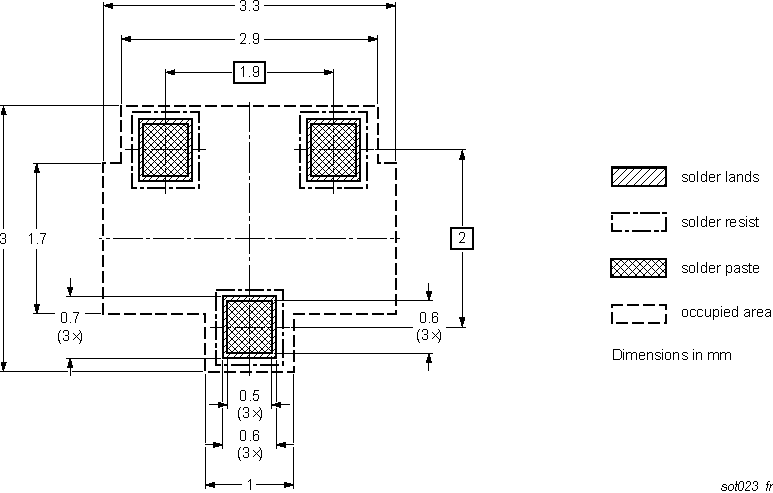
\includegraphics[width=1\linewidth]{bilder/sot23footprint.pdf}
			\caption{Transistor- Dimensionen als SOT23 Geh�uses, \\Quelle: NXP - PDTC114E Datenblatt S.10 }
			\label{fig:Messaufbau}
	\end{minipage}
	\hspace{1cm}
	\begin{minipage}[!ht]{0.45\textwidth}
		\centering 
		\captionsetup{type=figure}
		%\def\svgwidth{200pt}
		%\includegraphics[width=1\linewidth]{bilder/grafik_messaufbau.pdf}
		%	\includegraphics{bilder/messstand_biegebalken}
		%\resizebox{1.02\textwidth}{!}{\input{bilder/grafik_messaufbau.pdf_tex}}
		\caption{Informationsverlauf des Messaufbaus}
		\label{graf:Invormationsverlauf_Messaufbau}
	\end{minipage}
\end{center}

			% Vorl�ufige Gliederung
	\newpage
\chapter{Anordnung der Transistoren und Widerst�nde}
Das zu simulierende Modell  wurde daraufhin vereinfacht, dass die einzelnen Bauelemente durch Quader Repr�sentiert werden. Des weiteren wurde auf die Erstellung der Leiterbahnen verzichtet. Dadurch ergibt sich, dass die Leiterplatte ebenfalls durch einen einfachen Quader erstellt wird. Des Weiteren ist bei der Positionierung darauf zu achten, dass die abst�nde zwischen den Bauelementen in X-Richtung und in Y-Richtung Gleich gro� ist und innerhalb der Optimierung symmetrisch erweitert und verringert wird. 

\section{Transistoranordnung}
	Die Abbildung \ref{fig:Abmessungen_sot23} zeigt die Abmessungen eines Transistors der geforderten Bauform SOT23. Der Quader, welcher einen solchen Baustein repr�sentieren soll, erh�lt die darauf beruhenden Abmessungen h=1,1mm b=1,4mm h=3,0mm.
	\begin{center}
		\begin{minipage}[!ht]{0.8\textwidth}
			\captionsetup{type=figure}
			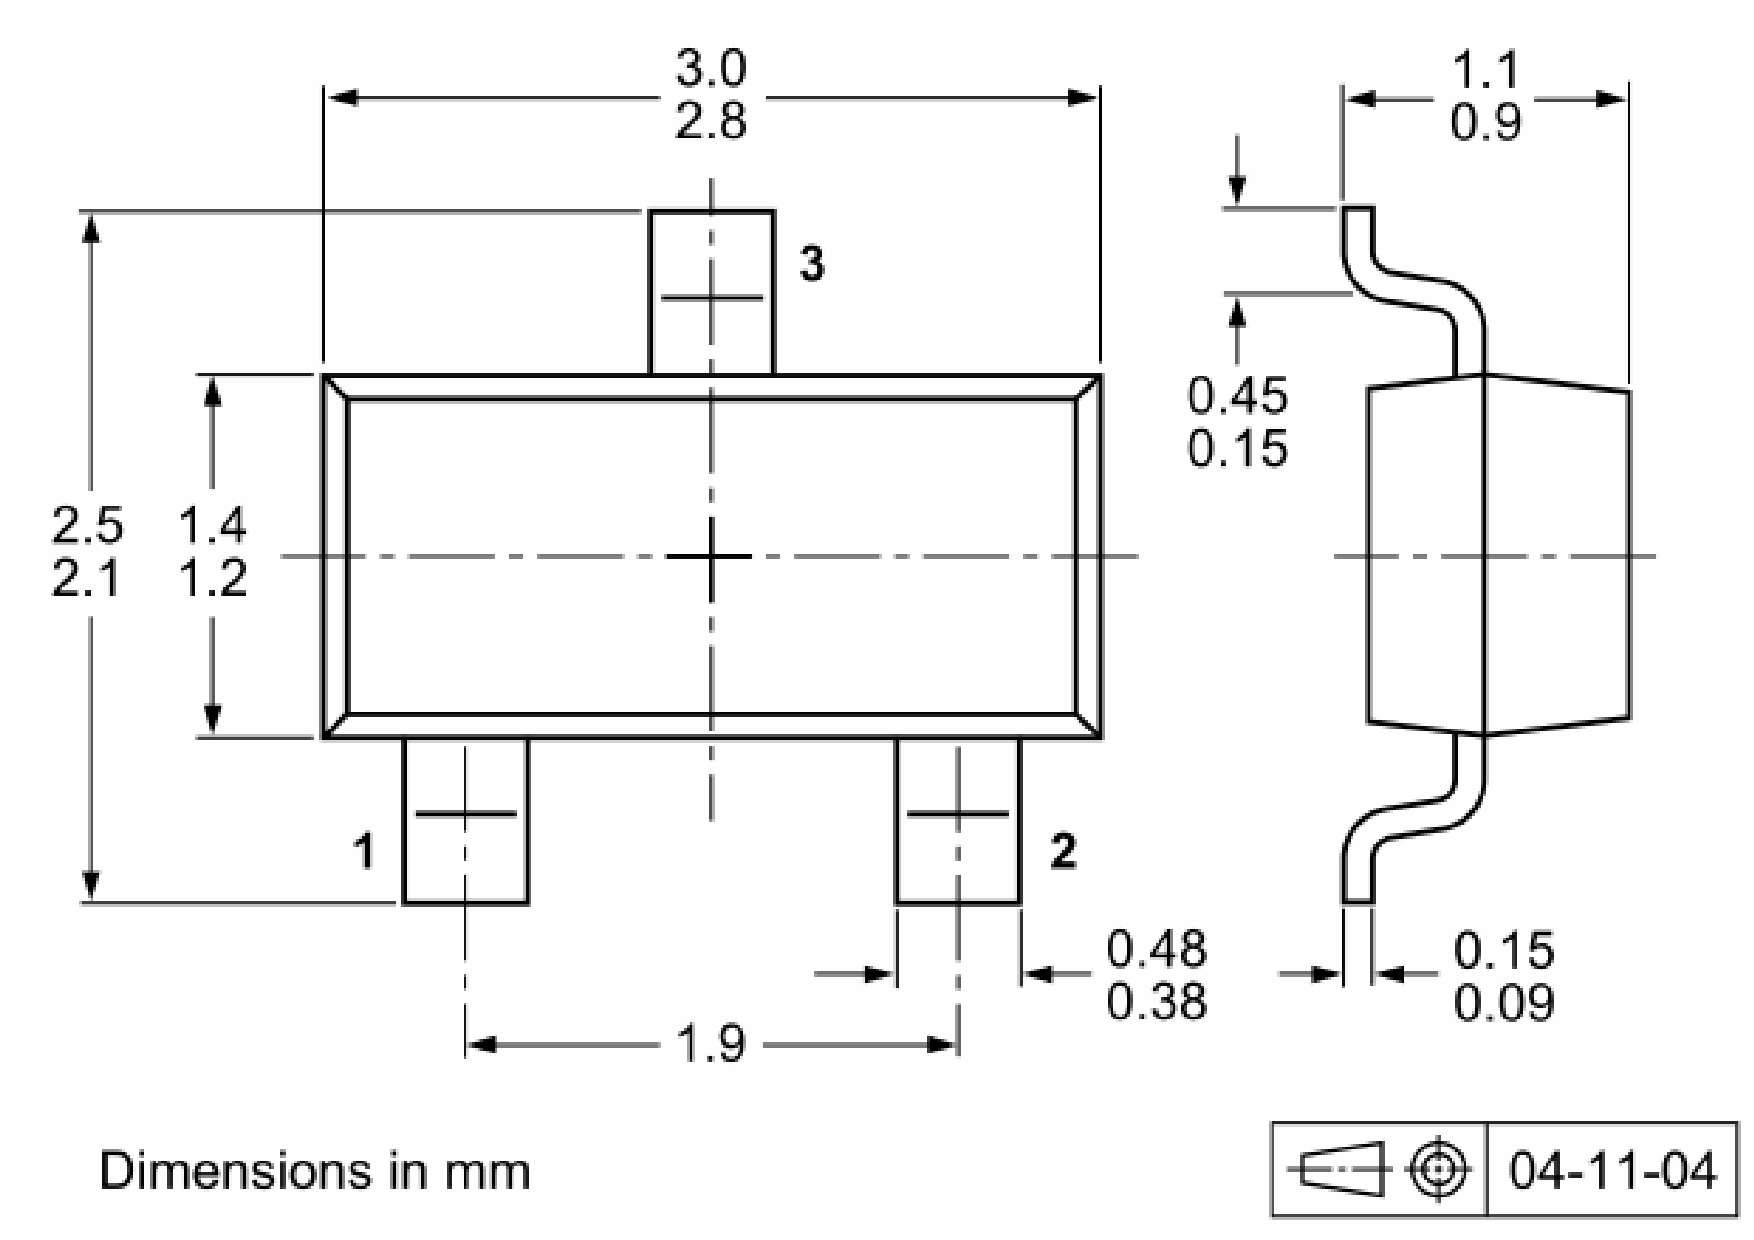
\includegraphics[width=1\linewidth]{bilder/Abmessungen_SOT23}
			\caption{Transistor - Abmessungen eines SOT23 Geh�uses, Quelle: NXP - PDTC114E Datenblatt S.10}
			\label{fig:Abmessungen_sot23}
		\end{minipage}
	\end{center}
	Um die Transistoren zu Positionieren, muss die Gr��e der Anschl�sse ber�cksichtigt werden. diese wiederum werden �ber die footprints ermittelt. (vgl. Abbildung \ref{fig:footprint_sot23} ) Somit ergibt sich ein Mindestabstand zwischen den Mittelpunkten der Transistoren in Y-Richtung von 3 mm und in X-Richtung von 3,3 mm. Um nunmehr die Abst�nde synchron zu halten werden die Abst�nde in X-Richtung um weitere 1,6 mm Vergr��ert. Schlussendlich ergeben sich folgende Mindestabst�nde bzw. Vorgabelabst�nde f�r die Mittelpunktabst�nde:  
	\begin{table}[bh]
		\centering
		\caption{Abst�nde zwischen den Mittelpunkten der Transistoren}
		\begin{tabular}{l >{\centering\arraybackslash}p{4cm} >{\centering\arraybackslash}p{4cm} } 
			\rowcolor[gray]{.8} & Mittelpunktabstand in Y-Richtung & Mittelpunktabstand in X-Richtung\\
			Mindestgeh�useabstand = 0 mm& 4,6 mm & 3,3 mm\\	
			\rowcolor[gray]{.8}Sollgeh�useabstand = 2 mm& 6,6 mm & 5,3 mm\\
		\end{tabular}
		\label{tab:Abst�nde SOT23}
	\end{table}
	
\section{Dimensionierung der Widerst�nde}
	Die Abbildung \ref{fig:Abmessungen_SMD_1206} zeigt die Abmessungen der geforderten Widerst�nde. Hierbei ergeben sich die Abmessungen h=0,55 mm b=1,6 mm l=3,1 mm f�r das zu simulierende Modell. Die footprints legen einen Mindestabstand fest, somit muss rund um den Baustein ein abstand von 1,6 mm eingehalten werden.
	\begin{center}
		\begin{minipage}[!ht]{0.8\textwidth}
			\captionsetup{type=figure}
			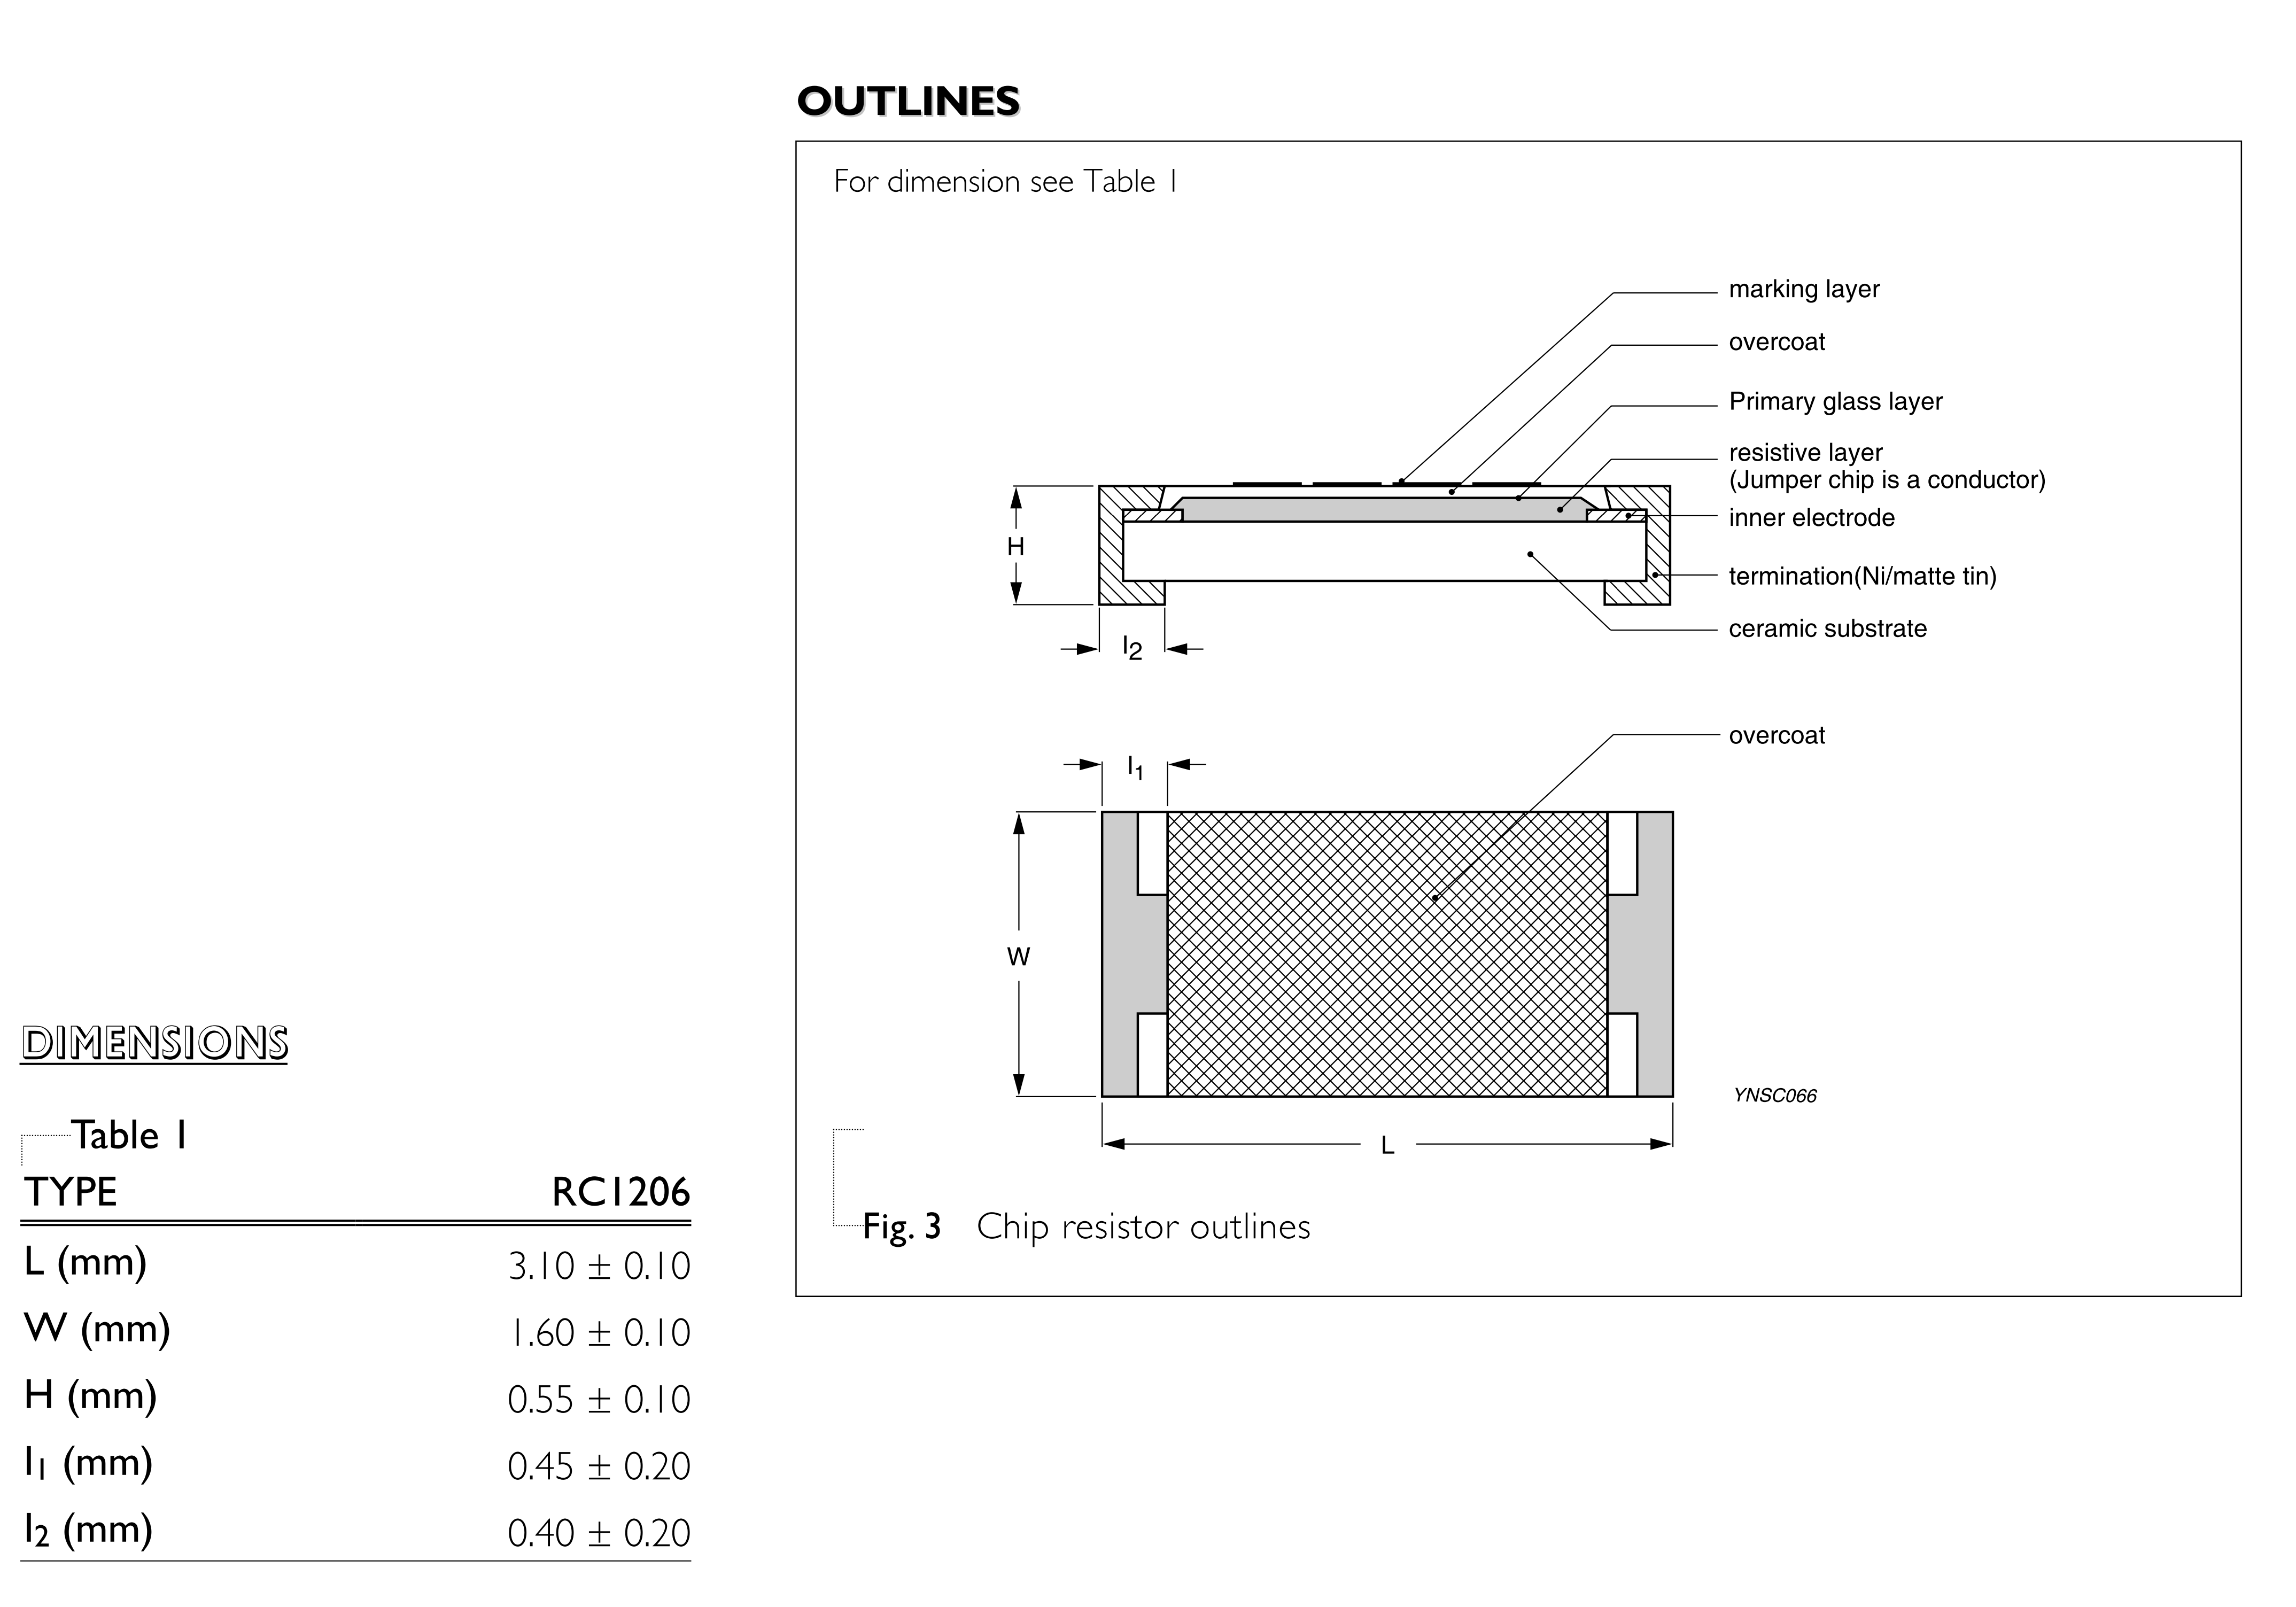
\includegraphics[width=1\linewidth]{bilder/Abnessungen_SMD_1206}
			\caption{Widerstand - Abmessungen SMD 1206, Quelle: Datenblatt RC1206 S.4}
			\label{fig:Abmessungen_SMD_1206}
		\end{minipage}
	\end{center}
	\newpage
	Weiter ergeben sich somit folgende Mittelpunktabst�nde:
	\begin{table}[bh]
		\centering
		\caption{Abst�nde zwischen den Mittelpunkten der SMD Widerst�nde}
		\begin{tabular}{l >{\centering\arraybackslash}p{4cm} >{\centering\arraybackslash}p{4cm} } 
			\rowcolor[gray]{.8} & Mittelpunktabstand in Y-Richtung & Mittelpunktabstand in X-Richtung\\
			Mindestgeh�useabstand = 0 mm& 4,6 mm & 3,2 mm\\	
			\rowcolor[gray]{.8}Sollgeh�useabstand = 2 mm& 6,6 mm & 5,2 mm\\
		\end{tabular}
		\label{tab:Abst�nde SOT23}
	\end{table}
\section{Bildung des zu simulierenden Modells}
	Mit den zuvor angegebenen Vorgaben wurden die folgenden Geometrien geschaffen. Dabei wird auf der Platine ein Bauelement generiert und dieses �ber eine zweifache Anwendung der Muster-Funktion zu einer Matrix erweitert.
	Ein selbst gesetztes Ziel ist es hierbei, die Matrix mit einem Parameter editieren zu k�nnen. Dabei sind die Abst�nde in X- und Y-Richtung Unterschiedlich. Das Problem wurde folgender Ma�en gel�st:
	Im ersten Schritt wurde ein Parameter P20 erzeugt, welcher den geringeren Abstand zwischen den Mittelpunkten zwei benachbarter Bauelemente beschreibt. Dieser soll sp�ter ge�ndert werden. Um diesen nun mit dem Abstand verkn�pfen zu k�nnen, wurde ein Parameter mit der L�nge 1,0 mm geschaffen. Somit kann der Abstand durch das Produkt der Parameter gewonnen werden. Um die unterschiedlichen Abst�nde in X- und Y-Richtung zu realisieren, wurde ein Offset-Parameter geschaffen, der nun mit dem anderen Abstand addiert wird. Da dieser wiederum von dem Parameter P20 Abh�ngt, sind beide Abst�nde von diesem Parameter abh�ngig und trotzdem bleiben die Abst�nde zwischen den Bauelementen Symmetrisch. Im folgenden werden die Geometrien f�r die Simulation der Transistoren gezeigt.
	\begin{center}
		\begin{minipage}[!ht]{0.6\textwidth}
			\captionsetup{type=figure}
			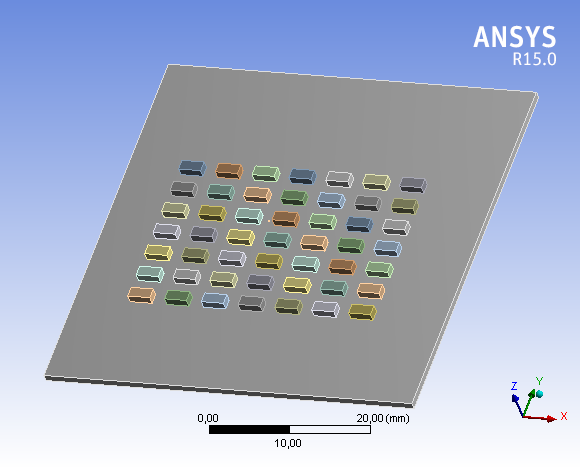
\includegraphics[width=1\linewidth]{bilder/TransistorMatrix}
			\caption{Transistor - Matrix}
			\label{fig:TransistorMatrix}
		\end{minipage}
	\end{center}
	und im Vergleich dazu die Matrix der Widerst�nde.
	\begin{center}
		\begin{minipage}[!ht]{0.6\textwidth}
			\captionsetup{type=figure}
			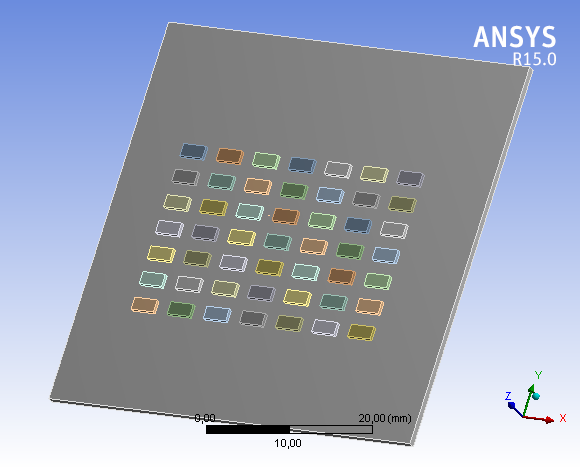
\includegraphics[width=1\linewidth]{bilder/WiderstandsMatrix}
			\caption{Widerstand - Matrix}
			\label{fig:WiderstandsMatrix}
		\end{minipage}
	\end{center}
	Zu erkennen ist, dass sich die beiden Geometrien haupts�chlich durch die Bauteilh�he des SOT23-Geh�uses und der SMD-Widerstandes 1206 unterscheiden. Die Matrizen und Abst�nde zwischen den Bauteilen �hneln sich.
\chapter{Thermisch station�re Simulation}
	Nachdem Die Geometrie definiert ist (Siehe Abschnitt  ) m�ssen verschiedene Messpunkte definiert werden. Um die Aufgabenstellung zu erf�llen m�ssen Messpunkte auf zwei aktive Bauelemente gesetzt werden und ein Messpunkt zwischen diesen Pixeln.  Mit diesen Messwerten kann nun in einem separaten Parameter die Differenz von Pixeltemperatur zu Pixelzwischenraumtemperatur gebildet werden. Dieser wird in einer sp�teren Optimierung ben�tigt. 
	Im Zuge dieser Messpunktdefinition, soll mittig zwischen den Pixeln ein Messpunkt definiert sein. Um diese Anforderung zu entsprechen wurde wie folgt vorgegangen:
	\begin{itemize}
		\item Erstellung eines Koordinatensystems zwischen den Auflagefl�chen zweier Bauteile
		\item Erstellen einer Skizze eines Quadrates Symmetrisch um den Ursprung des geschaffenen Koordinatensystems
		\item Extrudieren der Skizze so, dass eine kleine Schicht der Platine entfernt wird (0,1 mm)
	\end{itemize}
	Durch dieses vorgehen wird eine kleine Fl�che geschaffen, die auch bei �nderung des Bauteilabstandes, mittig der beiden Bauelemente, definiert ist. Daraufhin kann auf diese geschaffene Fl�che ein Messpunkt gesetzt werden. Der erzeugte Ausschnitt ist dabei so gering definiert, dass es die thermischen Eigenschaften der Leiterplatte kaum beeinflusst.
	Nachteil dieser L�sung ist, dass  das Netz nicht mehr gleichm��ig definiert wird.
	
	Weiterf�hrend wurde folgende Parameter gesetzt, um eine Optimierung durchf�hren zu k�nnen.
	\begin{itemize}
		\item Maximale Temperatur
		\item maximale Temperatur �u�erer Pixel der oberen Reihe
		\item maximale Temperatur mittlerer Pixel der oberen Reihe
		\item maximale Temperatur zwischen den genannten Pixeln
		\item maximale Temperatur passiver Pixel
		\item Abstand der Pixelmittelpunkte
		\item Wert der internen W�rmeerzeugung
	\end{itemize}
	
	Folgend werden die Vernetzung und die Definition der Aktiven Pixel gezeigt:
	
	\begin{LARGE}
		TODO: Bild Netz
		
		TODO: Bild Interne W�rmeerzeugung	
	\end{LARGE}
	
	Des weiteren wurden Folgende thermischen Senken bzw. Beziehungen definiert:
	
	\begin{table}[bh]
		\centering
		\caption{Eigenschaftsdefinition der Fl�chen}
		\begin{tabular}{p{5cm}  p{5cm}  c } 
			\rowcolor[gray]{.8} thermische Eigenschaft & Anwendung auf:& Wert\\
			Konvektion& alle Fl�chen & 8 $ \dfrac{W}{m^{2}} $	\\	
			\rowcolor[gray]{.8}Strahlung auf Umgebung & Oberfl�che der Platine & ---\\
			Strahlung auf Nachbarfl�chen & Oberfl�chen der Bauelemente '(Pixel) & ---
		\end{tabular}
		\label{tab:Eigenschaftsdefinition_der_Fl�chen}
	\end{table}
	
	\section{Simulation der Transistor Matrix}
	...
		\subsection{Optimierung}
		...
		\subsection{Aufgabe mit Rand}
		...
	\section{Simulation der Widerstandsmatrix}
	...
		\subsection{Optimierung}
		...
		\subsection{Aufgabe mit Rand}
		...
											% Grundlagen Kapitel einf�gen (grund.tex)
	%\chapter{Hardware-Realisierung}
\label{chpt:hardwarerealisierung}
F�r die Hardwarerealisierung sind verschiedenen Bedingungen zu beachten. Zum einen muss die Kompatibilit�t zur Messplatine gew�hrleistet, zum anderen die Leistungskenndaten der Schrittmotoren und die verf�gbare Spannungsversorgung ber�cksichtigt werden.
Weil zwei unterschiedliche Motoren zur Verf�gung stehen, werden nur die Kenndaten mit den h�heren Leistungskenndaten ber�cksichtigt. Die Steuerung kann dann auch f�r den anderen Motor verwendet werden.
%%%%%%%%%%%%%%%%%%
% Mikrocontroller
%%%%%%%%%%%%%%%%%%
\section{Mikrocontroller}
In der vorliegenden Messplatine f�r die Dehnungsmessstreifen, befindet sich ein \gls{avr} ATMega 8-Bit Mikrocontroller der Firma Atmel. Daher liegt es nahe, auch f�r die Schrittmotorsteuerung einen solchen Controller zu verwenden.
F�r die Schrittmotorsteuerung werden neben der I\textsuperscript{2}C-Schnittstelle zur Kommunikation auch zwei Timer ben�tigt. Die Steuerung des Treiber-ICs erfordert sechs Input-Out-Pins (IO-Pins), f�r die geplante Stromregelung m�ssen zwei Analog-Digital-Converter-Kan�le (ADC-Kan�le) eingeplant werden. Zur Programmierung sollte eine integrierte Entwicklungsumgebung (IDE) und ein Programmierger�t zur Verf�gung stehen. 

Ein \gls{arm}-Controller w�re f�r diese Aufgabe auch geeignet. Sehr viele Hersteller produzieren \gls{arm}-Controller und damit auch ihre eigenen Besonderheiten. Der ARM-Controller verf�gtin der Regel �ber einen gr��eren Speicher, mehr Peripherie und mehr Rechenleistung. F�r die Schrittmotorsteuerung ist keine hohe Komplexit�t zu erwarten und des Weiteren ist die Einarbeitung in die Architektur sehr zeitaufwendig, daher wird auf einn \gls{avr}-Controller zur�ck gegriffen. Hier liegt ein breites Spektrum von Atmel vor. 


Eine weitere wichtige Anforderung ist das Vorhanden sein einer Programmierschnittstelle und eines geeigneten Programmier- und Debugwerkzeuges. F�r Atmel-Mikrocontroller ist daf�r die \gls{jtag}-Schnittstelle oder ein \gls{isp}-Programmer notwendig. In Tabelle \ref{tab:Gegen�berstellungMindesanforderungen} ist ein Vergleich zwischen den Mindestanforderungen und einer kleinen Auswahl an Mikrocontrollern dargestellt. Die �bersicht zeigt recht deutlich, dass f�r die Motorsteuerung theoretisch auch einer der bekanntesten Mikrocontroller von Atmel, der ATMega8, ausreichen w�rde. Auf Grund von Sammelbestellungen und dem Vorliegen eines In-System-Debuggers wird der angegebene ATMega324P verwendet.
\begin{table}
	\centering
		\caption{Mindestanforderungen und Eigenschaften der Mikrocontroller}
		\begin{tabular}{c c c c c}
		\textbf{Eigenschaften}	& \textbf{Anforderung} & \textbf{ATmega324P} 	 					&\textbf{ATmega8}	\\\hline
	IO-Pins							&				9			&			32								&	23 			\\
\rowcolor[gray]{.8}	I\textsuperscript{2}C		&			1		&			1									& 1  			\\
	ADC-Kan�le							&				2			&			8							& 8				\\
\rowcolor[gray]{.8}	Timer											&			2			&   3											&	3				\\
 	Spannungsversorgung				&		$5 \, \mathrm{V}$	&		$1,8\, \mathrm{V} - 5,5\, \mathrm{V}$	&$2,7\, \mathrm{V} - 5{,}5\, \mathrm{V}$ \\
\rowcolor[gray]{.8}  Programmierschnittstelle				&JTAG &	JTAG	&    ISP        \\
			\end{tabular}
	\label{tab:Gegen�berstellungMindesanforderungen}
\end{table}
%%%%%%%%%%%%%%%%%%
% H-Br�cke
%%%%%%%%%%%%%%%%%%
\section{H-Br�cke} \label{ch:hbrucke}
Wie in der Einleitung zu Kapitel \ref{chpt:hardwarerealisierung} beschrieben, wird die Schrittmotorsteuerung f�r die horizontale Fahrrichtung (Motor 1, siehe Tabelle \ref{tab:Motoreigenschaften}) dimensioniert.
Relevant ist hier der maximale Strom von $ 4{,}2 \, \mathrm{A} $ bei einer Spannung von $ 2{,}1 \; \text{V} $ (nach Rechnung (\ref{eq:phasenstrom}))
\begin{equation}
	U_{\text{Phase}}= 4{,}2 \, \mathrm{A} \cdot 0{,}5 \; \Omega = 2{,}1 \; \text{V}.
\label{eq:phasenstrom}
\end{equation}
Zur Energieversorgung stehen $24 \, \mathrm{V}$ und maximal $1 \, \mathrm{A}$ zur Verf�gung. Das hei�t, dass eine Stromregelung nach dem Buck-Converter-Prinzip am Motortreiber umgesetzt wird. Um f�r andere Anwendungen sp�ter eine Steuerung zur Verf�gung zu haben, sollte der Motor-Treiber (H-Br�cke) �berdimensioniert werden.


% Quelle mosfets ?
F�r die Schrittmotorsteuerung werden zwei H-Br�cken ben�tigt. Um den Schaltungsaufbau zu minimieren, wird ein integrierter Motortreiber (Texas Instruments: DRV8432) mit zwei H-Br�cken benutzt. Der DRV8432 arbeitet mit einer maximalen Betriebsspannung von $52 \text{ V}$ und kann einen Dauerstrom von $2 \text{ x } 7 \mathrm{A}$ ($2 \text{ x }12\text{ A}$ Spitzenstrom) liefern. Der Motor-Treiber kann eine PWM-Frequenz von bis zu $500 \text{ kHz}$ verarbeiten. 
Zus�tzlich besitzt der Motortreiber einen einstellbaren �berstromschutz und Selbst-Schutzmechanismen wie Unterspannungsschutz, \gls{otw}, �berladungsschutz und \gls{flt} \cite{TI:Datasheet}.

Um das eintreten eines Fehlerzustandes zu signalisieren, stellt der Treiber die Signale OTW und FAULT an den entsprechenden Pins bereit. 
Zur Auswertung wird sowohl f�r �berstrom als auch f�r �bertemperatur jeweils ein Pin (aktiv LOW) f�r den Mikrocontroller zur Verf�gung gestellt. Die PWM-Signaleing�nge m�ssen LVTTL-Pegel ($3,3 \text{ V}$) besitzen.

\paragraph{Varianten zur Strommessung mit Shunt}
$\,$

Eine M�glichkeit ist, die Strommessung �ber einen Shunt zu realisieren. Dieser befindet sich im Drainstrompfad und der Mikrocontroller kann die gemessene Spannung direkt auswerten. Eine weitere M�glichkeit den Strom eines Motors zu ermitteln, ist die direkte Messung des Phasenstroms. Dies hat zur Folge, dass sowohl positive als auch negative Spannungen gemessen werden, da der Strom in der Phase nach der Schrittfolge in unterschiedliche Richtungen flie�t. Ein Mikrocontroller kann aber nur positive Spannungen messen. Eine Signalaufbereitung durch eine Analogschaltung ist hierf�r notwendig. Diese zwei erw�hnten Messm�glichkeiten werden mit einem Shunt durchgef�hrt. Eine weitere M�glichkeit ist die Messung mittels eines Stromwandlers. Hier wird zwischen aktiven und passiven unterschieden. Der passive Stromwandler besteht aus einem Eisenring, wodurch der stromdurchflossene Leiter gewickelt ist (Prim�rwicklung). Eine weitere Wicklung (Sekund�rwicklung) ist mit einem Shunt verbunden. Der aktive Stromwandler wird ebenfalls mit einem Eisenring und zus�tzlich mit einem Hall-Sensor ausgef�hrt, welcher im Schlitz des Eisenringes eingef�gt ist. In beiden Arten wird das Magnetfeld des Leiters gemessen. Nachteil dieser Messmethoden ist ein erh�hter Schaltungsaufwand und die damit erh�hten Kosten, welche f�r die Strommessung am Schrittmotor nicht notwendig sind.

Zur Bestimmung des Stromes wird die Strommessung mittels Shunt im Drainstrompfad umgesetzt. Der \gls{adc} im Mikrocontroller wird auf eine Referenzspannung von $1,1 \text{ V}$ eingestellt. Die Wandlung der Spannung im ADC wird bei steigender Flanke des PWM-Signals getriggert. So ist gew�hrleistet, dass der Strom immer zum High-Signal der PWM gemessen wird. Weitere Erl�uterungen zur PWM werden in Kapitel \ref{sc:stromregelung} erl�utert. Der maximale Phasenstrom betr�gt $4,2 \text{ A}$. Der Shunt muss f�r folgende Leistung dimensioniert sein:
\begin{equation}
P= U \cdot I = 1,1 \text{ V} \cdot 4,2 \text{ A} =  4,62\,\text{ W}
\label{eq:pshunt}
\end{equation}
Es wird ein Shunt von VISHAY mit \SI{0,25}{\ohm} und \SI{5}{\text{ W}} maximaler Verlustleistung benutzt. Der Widerstand besitzt ein Thermalpad auf der Oberseite, dass hei�t es besteht die M�glichkeit mit einem zus�tzlichem K�hlk�rper die maximal m�gliche Verlustleistung zu erh�hen. 
%%%%%%%%%%%%%%%%%%
% Pegelwandler
%%%%%%%%%%%%%%%%%%
\section{Pegelwandler}
Der Mikrocontroller wird mit $5\text{ V}$ betrieben, das hei�t, dass die IO-Ausg�nge ebenfalls diese Spannung besitzen. Der Motortreiber DRV8432 darf aber nur mit LVTTL betrieben ($3,3 \text{ V}$) werden, da die PWM-Signaleing�nge nicht $5\text{ V}$ Spannungsfest sind. Folglich muss der Spannungspegel angepasst werden. Der Pegelwandler muss  $5\text{ V}$  eingangstolerant sein und darf nicht f�r Push-Pull und Open-Drain-Betrieb ausgelegt sein (siehe Abbildung \ref{fig:pegel0}). 
\begin{figure}[h!]%Quelle: LT-Spice
			\centering
			\includegraphics[width=0.4\linewidth]{bilder/pegelwandler0.pdf}
			\caption{Signal\"ubertragung zwischen Mikrocontroller und Motortreiber ohne Pegelwandlung (vlg. \cite{MT:TipsAndTricks} S.127)}
			\label{fig:pegel0}
\end{figure}

Die Pegelwandlung kann �ber einen Spannungsteiler (siehe Abbildung \ref{fig:pegel1}) realisiert werden. Je nach ben�tigter �bertragungsgeschwindigkeit und Belastung des Ausganges vom Mikrocontroller muss der Spannungsteiler richtig Dimensioniert werden. 
\begin{figure}[h!]%Quelle: LT-Spice
			\centering
			\includegraphics[width=0.4\linewidth]{bilder/pegelwandler1.pdf}
			\caption{Pegelanpassung mittels Spannungsteiler (vlg. \cite{MT:TipsAndTricks} S.128)}
			\label{fig:pegel1}
\end{figure}

Eine weitere M�glichkeit ist eine Klemmdiode am $3,3\text{ V}$-Eingang. Um den Strom durch die Diode gering zu halten, muss ein Vorwiderstand hinzugef�gt werden. Dieser besitzt den Nachteil, dass der Spannungspegel eventuell nicht so schnell wie gew�nscht umgewandelt wird (siehe Abbildung \ref{fig:pegel2}). Ein weiterer Nachteil einer Klemmdiode ist, dass Strom in den $3,3\text{ V}$-Eingang gespeist wird. Abhilfe schafft ein Transistor der den Strom an die Masse abf�hrt (siehe Abbildung \ref{fig:pegel3}).
\begin{center}
	\begin{minipage}[!ht]{0.47\textwidth}
			\captionsetup{type=figure}
			\includegraphics[width=0.9\linewidth]{bilder/pegelwandler2.pdf}
			\caption{Pegelanpassung mittels Diode (vlg. \cite{MT:TipsAndTricks} S.127)}
			\label{fig:pegel2}
	\end{minipage}
	\quad
	\begin{minipage}[!ht]{0.47\textwidth}
			\captionsetup{type=figure}
			\includegraphics[width=0.9\linewidth]{bilder/pegelwandler3.pdf}
			\caption{Pegelanpassung mittels Transistor (vlg. \cite{MT:TipsAndTricks} S.128)}
			\label{fig:pegel3}
	\end{minipage}
\end{center}

F�r den verwendeten Motortreiber m�ssen insgesamt sechs Signale auf $3,3\text{ V}$ gewandelt werden. Vier zur Generierung des Drehfeldes an den zwei Phasen des Schrittmotors und zus�tzlich zwei Signale zum Ein- und Ausschalten der Phasen. Ein diskreter Aufbau, wie die beschriebenen L�sungen f�hren bei Anpassung mehrerer Signale zu einem erh�hten Schaltungsaufwand \cite{MT:TipsAndTricks}. Durch eine \gls{ic} l�sst sich dieser minimieren (siehe Abbildung \ref{fig:pege4}). Das hei�t, anstatt mehrere kleinere passive Bauelemente zu verschalten wird nur ein aktives Bauteil verwendet. Hierf�r wird der 74LVC245A von TI eingesetzt \cite{TI:DatasheetLT}. 
\begin{figure}[h!]%Quelle: LT-Spice
			\centering
			\includegraphics[width=0.6\linewidth]{bilder/pegelwandler4.pdf}
			\caption{Pegelanpassung mittels Pegelwandler 74LVC245A}
			\label{fig:pege4}
\end{figure}

\begin{center}
	\begin{minipage}[!ht]{0.49\textwidth}
			\centering
			\captionsetup{type=figure}
			\includegraphics[height=4cm]{bilder/74LVC245A.pdf}
			\caption{Pinbelegung 74LVC245A, \\(vgl. \cite{TI:DatasheetLT} S.1)}
			\label{fig:pegel5}
	\end{minipage}
	\begin{minipage}[!ht]{0.49\textwidth}
			\captionsetup{type=figure}
			\includegraphics[height=4cm]{bilder/74LVC245A_1.pdf}
			%\includegraphics[0,0][20,80]{bilder/74LVC245A_1.pdf}
			\caption[Logikplan 74LVC245A]{Logikplan 74LVC245A, \\(vgl. \cite{TI:DatasheetLT} S.2)}
			\label{fig:pegel6}
	\end{minipage}
\end{center}

Dies ist ein Bustreiber mit $5\text{ V}$ toleranten Eing�ngen und wird in der Schaltung als Pegelwandler verwendet. Er kann in Abh�ngigkeit des Logikpegels am Richtungspin (DIR) Signale von Seite A zu B oder umgekehrt �bertragen. Der Ausgangsspannungsbereich liegt zwischen $1,65\text{ V}$ und $ 3,6\text{ V}$ \cite{TI:DatasheetLT}. In Tabelle \ref{tab:fktitabelpegel} sind die drei Zust�nde des Pegelwandlers in Abh�ngigkeit der Logikpegel an den Eing�ngen beschrieben, zus�tzlich ist der Logikplan aufgezeichnet (siehe Abbildung \ref{fig:pegel6}).

\begin{table*}[!h]
	\centering
	\caption[Funktionstabelle 74LVC245A, \\H-High, L-Low, X-Tristate]{Funktionstabelle 74LVC245A, \\H-High, L-Low, X-Tristate, (vgl. \cite{TI:DatasheetLT} S.2 )}
		\begin{tabular}{c c c}
		\multicolumn{2}{c}{\textbf{Eing�nge}}			& {\textbf{Operation}} \\
	$\overline{\text{OE}}$		&	DIR			&			\\\hline
	\rowcolor[gray]{.8} L												& L 			&		Datentransfer von B nach A	\\
	L													&	H				&		Datentransfer von A nach B				\\
\rowcolor[gray]{.8}	H													& X				&		Isolation			\\
 			\end{tabular}
	\label{tab:fktitabelpegel}
\end{table*}

%%%%%%%%%%%%%%%%%%%%%%%%%%%%%%%%%%%%%%%%%%%%%%%%%%
%%%%%%%%%%				Spannungsversorgung
%%%%%%%%%%%%%%%%%%%%%%%%%%%%%%%%%%%%%%%%%%%%%%%%%%
\newpage
\section{Spannungsversorgung}
F�r die gesamte Schaltung sind unterschiedliche Spannungen notwendig. Vom Netzteil werden  $24\text{ V}$ direkt f�r die PVDD (Spannung des Leistungsteils vom DRV8432) und  $5\text{ V}$ direkt f�r den Mikrocontroller zur Verf�gung gestellt.
Der Motortreiber ben�tigt $12 \text{ V}$  f�r die VDD (Spannungsversorgung vom DRV8432) und f�r die GVDD (Gatespannung vom DRV8432) mit einer maximalen Stromaufnahme von  $18,5 \text{ mA}$, der Pegelwandler ben�tigt $3,3 \text{ V}$ und $\pm 50 \text{ mA}$. Diese Spannungen werden durch Linearregler gewandelt (siehe Tabelle \ref{tab:spanungsversorgung}), aus $24 \text{ V}$ werden $12 \text{ V}$ und aus $5 \text{ V}$ werden $3,3 \text{ V}$ erzeugt. Wie im Kapitel \ref{sec:buckconvert} beschrieben ist der Wirkungsgrad von Linearregler nicht sehr gro�, da sie die �bersch�ssige Energie in W�rme umwandeln. Da keine gro�en Str�me gewandelt werden, sind die Verluste vernachl�ssigbar klein.
\begin{table*}[!h]
	\centering
	\caption{Spannungsversorgung der ICs}
		\begin{tabular}{r c r}
					Bauelelement										&  Versorgungsspannung & Bauteil						\\ \hline
				IO-Mikrocontroller								&				$5\text{ V}$						&	Netzteil					\\
				\rowcolor[gray]{.8}	Motortreiber PVDD	&		 $24\text{ V}$		& Netzteil					\\
				\rowcolor[gray]{.8}				VDD,	GVDD	&		 $12\text{ V}$	&			LM3490IM5-12	\\
				\gls{adc}-Pegelwandler						&		$3,3 \text{ V}$							& LM3480IM3-3.3			\\
 			\end{tabular}
		\label{tab:spanungsversorgung}
\end{table*}

	%
	%\chapter{Software-Realisierung}
Die Software f�r  den Mikrocontroller wird in ANSI C geschrieben und gliedert sich in drei Hauptbestandteile: Schrittgenerierung, Stromregelung, Kommunikation (I\textsuperscript{2}C).

\section{Schrittgenerierung}

Die Schrittgenerierung (Phasengenerierung) erfolgt �ber dem in Kapitel \ref{sec:MAnsteuerung} beschriebenen Ablauf. Nach dem letzten Schritt wiederholt sich der Ablauf, so dass die State Machine aus vier Zust�nden besteht (siehe Abbildung \ref{fig:statemachine}). 
Der Zustandsautomat wird in der Interrupt-Service-Routine (ISR) des Timer 2 als Switch-Case-Anweisung abgearbeitet. 
Die Frequenz (f) des Timers ist �quivalent der Drehzahl (n) des Motors und abh�ngig von der Schrittweite ($\alpha$). 
\begin{equation}
n = f \cdot 60 \cdot \frac{\alpha}{360} \qquad[n]=\frac{1}{\text{min}} \quad [f]=\text{Hz}
\label{eq:freqdreh}
\end{equation}
Soll zwischen Vorw�rts- ($\text{v}$) und R�ckw�rtsdrehung ($\overline{\text{v}}$) unterschieden werden, l�uft der Zustandsgraph gegen den Uhrzeigersinn ab. Die Richtung und die Schrittfrequenz wird vom Kraftregler an die Schrittmotorsteuerung �bergeben.

%Quelle: LT-Spice
\begin{center}
			\captionsetup{type=figure}
			\input{bilder/statemachine_0.pdf_tex}
			\caption{State Machine}
			\label{fig:statemachine}
\end{center}

\section{Stromregelung}\label{sc:stromregelung}
Um eine Stromregelung zu generieren, wird die Ansteuerung nach dem Buck-Converter-Prinzip vorgenommen (siehe Kapitel \ref{sec:buckconvert}). Das hei�t, dass zus�tzlich zu den vier Zust�nden der Ausg�nge ein PWM-Signal �berlagert wird \mbox{(siehe Abbildung \ref{fig:pwm})}.
Das PWM-Signal wird im Timer 0 erzeugt und l�uft mit einer Frequenz von 78,125~kHz. Um die �berlagerung zu gew�hrleisten, wird das PWM-Signal herausgef�hrt und �ber ein UND-Glied mit den Signalen aus der State Machine konjunktiv verkn�pft.

\begin{figure}[h!]%Quelle: LT-Spice
			\centering
			\input{bilder/pwm1.pdf_tex}
			\caption{Prinzipielle Darstellung der �berlagerung von der PWM und der Schrittgenerierung}
			\label{fig:pwm}
\end{figure}

\newpage
\subsection{Theoretische Vorbetrachtung}
F�r die theoretische Bestimmung der Regelparameter wird eine Vorbetrachtung der Regelstrecke in MATLAB/Simulink durchgef�hrt. Wie im Kapitel \ref{ch:hbrucke} beschrieben, wird der Strom �ber eine Spannungsmessung am Shunt mit $\SI{0,25}{\ohm}$ ermittelt. Es wird in allen Diagrammen nur die Spannung angezeigt, sie kann jeder Zeit in den Strom umgerechnet werden. In Abbildung \ref{graf:sprungantwort} ist die Sprungantwort f�r den Schrittmotor dargestellt. Es wurde ein Spannungssprung mit $1 \text{ V}$ bei $0,010\text{ s}$ auf die Strecke gegeben. Die Sprungantwort ist die Spannung am Shunt. Die Strecke ist in Abbildung \ref{graf:reglkreis}, mit der Wicklungsimpedanz ($L_\text{i} = 1,6 \text{ mH}$, $R_\text{i} = 0,5\,\Omega$), dem Messwiderstand ($R_\text{mess} = 0,25\,\Omega$) dargestellt.
%
% Sprungantwort Motor
%
%\begin{figure}[!h]%
\begin{center}
	\begin{tikzpicture}
		\begin{axis}[	width=0.9\textwidth,
									height=0.5\textwidth,
									% % % % % % % % X-Achse
									xmin=0,
									xmax=0.03,
									xtick={0.010,0.015,0.020,0.025,0.030},
									xticklabel style={%
													/pgf/number format/.cd,
													fixed,
													fixed zerofill,
													precision=3,
									},
									xlabel={$t/\text{s}$},
									% % % % % % % % Y-Achse
									%ymin=0,
									%ymax=0.4,
									yticklabel style={%
													/pgf/number format/.cd,
													fixed,
													fixed zerofill,
													precision=1,
													set thousands separator={},
									},
									ylabel={$U/\text{V}$},
									% % % % % % % %  Legende
									legend style={at={(0.97,0.03)},anchor=south east,draw=black,fill=white,legend cell align=left}
									]
 			%\addplot [color=blue,solid]table[row sep=crcr] {matlab/sprungantwort1.csv};
			%\addlegendentry{Spannungssprung auf 1 V};
			\addplot [color=black!50!green,solid]table[row sep=crcr]{matlab/sprungantwort2.csv};
			\addlegendentry{Spannungsantwort};
		\end{axis}
	\end{tikzpicture}
		\captionsetup{type=figure}
		\caption{Schrittmotor Sprungantwort }%
		\label{graf:sprungantwort}%
\end{center}



%\begin{center}
	%\centering
	%\input{matlab/Schrittmotor_Sprungantwort_2.tex}
	%\captionsetup{type=figure}
	%\caption{Schrittmotor Sprungantwort}%
	%\label{graf:sprungantwort}%
%\end{center}	
%\end{figure}
%\input{matlab/Schrittmotor_Sprungantwort.tex}
Die Grafik zeigt f�r den Motor ein PT1-Verhalten. Der Beharrungswert stellt sich bei $0,33 \text{ V}$ nach $0,03\text{ s}$.
Die Streckenverst�rkung berechnet sich aus dem Quotienten der Ist-Wert�nderung $\Delta x$ (Spannungssprung am Eingang) und der Soll-Wert�nderung $\Delta y$ (Beharrungswert der Spannung am Ausgang)
\begin{equation}
	k_s=\frac{\Delta x}{\Delta y}=\frac{0 \text{ V} 0,33 \text{ V}}{0 \text{ V} - 1 \text{ V}} = 0,33\text{ }.
\label{eq:Streckenverst�rkung}
\end{equation}

Die Zeit beim erreichen von $0,63\,\%$ des Beharrungswertes betr�gt $T_{0,63} = 0,0023\;s$.
Daraus ergibt sich f�r die Regelstrecke die �bertragungsfunktion:
\begin{equation}
	G(s) = \frac{0,33}{1+ 0,0023 s \cdot s }.
\label{eq:uebertragungsfunktion}
\end{equation}

 
Es wird f�r die Regelung ein PI-Regler angewendet. Dieser hat, im Gegensatz zum P-Reger, durch den Integralanteil keine bleibende Regelabweichung. 
Der Regler besteht aus dem Proportionalglied mit dem Parameter $k_p$ und dem Integralglied mit dem Parameter $k_i$ 
\begin{equation}
	y(t)=k_p \cdot e(t) + k_i \cdot \int \limits_{0}^\tau \! e(\tau) \, d\tau \text{ .}
\label{eq:piregler}
\end{equation}
Die Bestimmung von $k_p$ und $k_i$ erfolgt �ber die Einstellregeln von \emph{Chien-Hrones-Reswick} f�r einen PI-Regler.
\begin{equation}
	k_p = \frac{0,35}{k_s}\cdot \frac{T_g}{T_u} 
\label{eq:chr1}
\end{equation}
\begin{equation}
k_i = k_p \cdot 1,2 \cdot T_g
\label{eq:chr2}
\end{equation}

\begin{center}
	\input{bilder/regelkreis_pi_wicklung.pdf_tex}
	\captionsetup{type=figure}
	\caption{Prinzipdarstellung des Regelkreises}%
	\label{graf:reglkreis}%
\end{center}


F�r die PT1-Strecke ist eine Ausgleichszeit $T_g = 0,0023 \text { s}$ aus Abbildung \ref{graf:sprungantwort}. ermittelt worden. Eine Verzugszeit $T_u$ ist nicht enthalten: sie wird deshalb f�r die Berechnung der Parameter als viel kleiner als die Ausgleichszeit angenommen: $T_u  <<  T_g$, d.h. \mbox{$T_u = 0,0001\text{ s}$}.
Eingesetzt in die Formeln \ref{eq:chr1} und \ref{eq:chr2} ergibt das f�r $k_p = 24.4$ und f�r $k_i = 0,0023$.
%
% Sprungantwort Regler
%

Der prinzipielle Aufbau des Regelkreises in Simulink ist in Abbildung \ref{graf:reglkreis} dargestellt. 
Der Beharrungswert stellt sich  nach $0,0076 \text{ s}$ ein (siehe Abbildung \ref{graf:fuehr_anal1}) und erreicht den SOLL-Wert nicht.
Durch den zuvor gestellte Annahme das $T_u  <<  T_g$ ist, war zu erwarten, dass die ermittelten Parameter noch nicht das Optimum darstellen.  
Um ein hinreichend schnelles Erreichen des Beharrungswertes zu gew�hrleisten, werden in der Simulation die Parameter angepasst.
Die Korrektur des Proportionalit�ts-Faktors hat die gr��te Auswirkung auf das F�hrungsverhalten. 95\% des SOLL-Wertes werden bei $t=0,025\text{ s}$ erreicht und der IST-Wert n�hert sich ihm weiter asymptotisch (siehe Abbildung \ref{graf:fuehr_anal2}).
%Es wird ein Sollwert (w) vorgeben und aus der Differenz mit der Strommessung die Spannung eingestellt. Das in Simulink simulierte F�hrungsverhalten des umgesetzten PI-Reglers ist in \mbox{Abbildung \ref{graf:Reglersprungantwort}} dargestellt. Nach $0,0105\text{ s}$ hat die Regelstrecke den Sollwert zu $90\%$ erreicht, der Beharrungswert stellt sich nach $0,002\text{ s}$ ein.
%\begin{center}
	%\input{matlab/Schrittmotor_Sprungantwort_Regler_1.tex}
	%\captionsetup{type=figure}
	%\caption{F�hrungsverhalten}%
	%\label{graf:Reglersprungantwort}%
%\end{center}
	\begin{figure}%
		\subfloat[\label{graf:fuehr_anal1} $k_\text{i}=0,0673$, $k_\text{p}=24,4$]{
			\begin{tikzpicture}
				\begin{axis}[	width=0.45\textwidth,
											height=.45\textwidth,
											% % % % % % % % X-Achse
											xmin=0,
											xmax=0.03,
											xtick={0.005,0.015,0.025},
											xticklabel style={%
															/pgf/number format/.cd,
															fixed,
															fixed zerofill,
															precision=3,
											},
											xlabel={$t/\text{s}$},
											% % % % % % % % Y-Achse
											ymin=0,
											%ymax=0.4,
											yticklabel style={%
															/pgf/number format/.cd,
															fixed,
															fixed zerofill,
															precision=1,
															set thousands separator={},
											},
											ylabel={$U_{R_{\text{mess}}}/\text{V}$},
											% % % % % % % %  Legende
											legend style={at={(0.97,0.03)},anchor=south east,draw=black,fill=white,legend cell align=left}
											]
					\addplot [color=blue,solid]table[row sep=crcr] {matlab/regler_sprung1.csv};
					\addlegendentry{SOLL-Wert};
					\addplot [color=black!50!green,solid]table[row sep=crcr]{matlab/regler_sprungantwort1.csv};
					\addlegendentry{IST-Wert};
				\end{axis}
			\end{tikzpicture}
			}
	%			\captionsetup{type=figure}
	%			\caption{$k_\text{i}=0.067344$, $k_\text{p}=24,4$ }%
	%			\label{graf:sprungantwort}%
	%	
	%\end{minipage}
	%\hspace{0.5cm}
	%\begin{minipage}[!ht]{0.49\textwidth}
	%	\begin{center}
		\subfloat[\label{graf:fuehr_anal2}$k_\text{i}=6000$, $k_\text{p}=24,4$]{
			\begin{tikzpicture}
				\begin{axis}[	width=.45\textwidth,
											height=.45\textwidth,
											% % % % % % % % X-Achse
											xmin=0,
											xmax=0.03,
											xtick={0.005,0.015,0.025},
											xticklabel style={%
															/pgf/number format/.cd,
															fixed,
															fixed zerofill,
															precision=3,
											},
											xlabel={$t/\text{s}$},
											% % % % % % % % Y-Achse
											ymin=0,
											%ymax=0.4,
											yticklabel style={%
															/pgf/number format/.cd,
															fixed,
															fixed zerofill,
															precision=1,
															set thousands separator={},
											},
											ylabel={$U_{R_{\text{mess}}}/\text{V}$},
											% % % % % % % %  Legende
											legend style={at={(0.97,0.03)},anchor=south east,draw=black,fill=white,legend cell align=left}
											]
					\addplot [color=blue,solid]table[row sep=crcr] {matlab/regler_sprung2.csv};
					\addlegendentry{SOLL-Wert};
					\addplot [color=black!50!green,solid]table[row sep=crcr]{matlab/regler_sprungantwort2.csv};
					\addlegendentry{IST-Wert};
				\end{axis}
			\end{tikzpicture}
			}
			\centering
			\caption{F�hrungsverhalten: \\a) nach berechneten Regelparametern\\ b) nach korrigierten Regelparametern }%
			\label{graf:fuehrungsverhalten}%
	\end{figure}
		%	\captionsetup{type=figure}
		%	\caption{$k_\text{i}=6000$, $k_\text{p}=24,4$}% }
		%	\label{graf:sprungantwort1}%
	%\end{center}
%\end{minipage}


F�r die Regelung im Mikrocontroller muss eine Diskretisierung vorgenommen werden. Der Motor 1 kann einen maximalen Strom von $4,2 \text{ A}$ aufnehmen. Zur Auswertung am Mikrocontroller kommt der ADC zum Einsatz. Der ADC-Wandler besitzt eine maximale Aufl�sung von $10$ Bit. Da die maximale Registerbreite des ATMega $8$ Bit betr�gt, wird der gewandelte Wert in zwei Register aufgeteilt. Die Rechnung mit einem $10$ Bit-Wert ist durch die Arbeit mit zwei Registern aufw�ndiger, deshalb wird eine Aufl�sung mit $8$ Bit bevorzugt. 
Die 10 Bit-Aufl�sung liefert eine Spannungsaufl�sung von \SI{0,001}{\volt}, eine Minimierung auf 8 Bit erzeugt eine Aufl�sung von \SI{0,004}{\volt} (siehe Tabelle \ref{tab:spanungsaufloesung}). Die resultierende Stromaufl�sung von \SI{0,004}{\A} bei 8 Bit ist f�r die Stromregelung ausreichend.
%\begin{align}
%\end{align}
\begin{table}[!h]
	\centering
		\caption{Spannungsaufl�sung}
		%\rowcolors{3}{gray}{yellow}
		\begin{tabular}{L{2cm}L{3.8cm}L{5cm}L{3cm}}
			\textbf{Aufl�sung}					& \textbf{Spannungs-aufl�sung} 						&	\textbf{resulitierende Stromaufl�sung}	& \textbf{Anzahl der Register}	\\ \hline
			$10$ Bit 										&$1,1 \text{ V}/2^{10}= \SI{0,0011}{\volt}$& $\SI{0,0011}{\volt}/\SI{0,25}{\ohm}=\SI{0,004}{\A}$	&	2									\\
			\rowcolor[gray]{.8}	$8$ Bit &$1,1 \text{ V}/2^{8}= \SI{0,0043}{\volt}$	&	$\SI{0,0043}{\volt}/\SI{0,25}{\ohm}=\SI{0,0172}{\A}$  &	1															\\
 		\end{tabular}
	\label{tab:spanungsaufloesung}
\end{table}

% % % % % % % % % % % % % % % % %
% Regler Diskretierung
% % % % % % % % % % % % % % % % %
Um eine m�gliche Umsetzung f�r den Mikrocontroller zu untersuchen, wird der zuvor simulierte Regler mit einer 8 Bit Aufl�sung in MATLAB/Simlink diskretisiert. 
Die Spannungswandlung f�r den ADC wird bei einer steigenden Flanke des PWM-Signals getriggert. So ist gew�hrleistet, dass der Strom immer im High-Abschnitt der PWM gemessen wird.
Die Samplefrequenz entspricht der PWM-Frequenz und betr�gt 78,125 kHz. In Abbildung \ref{graf:Reglersprungantwort_diskret} ist die diskretisierte Sprungantwort der Regelstrecke dargestellt. 
%\begin{center}
	%\input{matlab/Schrittmotor_Sprungantwort_diskret.tex}
	%\captionsetup{type=figure}
	%\caption{diskretisierte Sprungantwort auf 8 Bit}%
	%\label{graf:Reglersprungantwort_diskret}%
%\end{center}
%%%
% Diskretisierte SPrungantwort
%%%
\begin{center}
	\begin{tikzpicture}
		\begin{axis}[	width=0.8\textwidth,
									height=0.5\textwidth,
									% % % % % % % % X-Achse
									xmin=0,
									xmax=0.03,
									xtick={0.005,0.010,0.015,0.020,0.025,0.030},
									xticklabel style={%
													/pgf/number format/.cd,
													fixed,
													fixed zerofill,
													precision=3,
									},
									xlabel={$t/\text{s}$},
									% % % % % % % % Y-Achse
									ymin=0,
									ymax=85,
									yticklabel style={%
													/pgf/number format/.cd,
													fixed,
													fixed zerofill,
													precision=0,
									},
									ylabel={$U/(0,0043\cdot\text{V})$},
									% % % % % % % %  Legende
									legend style={at={(0.97,0.03)},anchor=south east,draw=black,fill=white,legend cell align=left}
									]
 			\addplot [color=blue,solid]table[row sep=crcr] {matlab/regler_digi_sprungantwort1.csv};
			\addlegendentry{diskretisierte Spannung};
		\end{axis}
	\end{tikzpicture}
		\captionsetup{type=figure}
		\caption{mit 8 Bit diskretisierte Sprungantwort }%
		\label{graf:Reglersprungantwort_diskret}%
\end{center}

Die diskrete Sprungantwort erreicht den Beharrungswert von $78{\text{ Digits}}$ nach $0,021\text{ s}$. Nach den Einstellregeln von \emph{Takahashi} f�r einen digitalen PI-Regler werden die Regelparameter berechnet. Die Parameter $k_s$ sowie $T_g$ und $T_u$ bleiben gleich, da sich die Strecke nicht ver�ndert hat. Auch die Annahme von $T_u << T_g$ wird f�r die Berechnung beibehalten, eine n�tige Anpassung der Parameter erfolgt in der Simulation. Die Abtastzeit wird aus der PWM-Frequenz berechnet, da sie die Spannungswandlung im ADC startet.


\begin{equation}
T_{Abtast} = \frac{1}{f_{\text{PWM}}} = 13,9 \text{ $\mu$s}
\label{eq:tkh3}
\end{equation}
\begin{equation}
	k_{p_{\text{diskret}}} = \frac{1}{k_s}\cdot \frac{0,9 \cdot T_g}{T_u+\frac{T_{\text{Abtast}}}{2}} = 58,12 
\label{eq:tkh1}
\end{equation}
\begin{equation}
k_{i_{\text{diskret}}}  = k_{p_{\text{diskret}}} \cdot 3,3 \cdot \left(T_u + \frac{T_{\text{Abtast}}}{2}\right)=0,021.
\label{eq:tkh2}
\end{equation}


F�r die berechnete Parameter ist das F�hrungsverhalten in Abbildung \ref{graf:fuehr_diskret1} dargestellt. Es ist deutlich zu erkennen, dass der Regler um den SOLL-Wert mit einer maximalen �berschwingweite von $12 \text{ Digits}$ schwingt. Nach Minimierung des Proportionalgliedes auf $k_{p_{\text{diskret}}} = 5$ senkt sich die maximale �berschwingweite auf $4$ Digits und es stellt sich der SOLL-Wert nach $0,01\text{ s}$ ein (siehe Abbildung \ref{graf:fuehr_diskret2}).

\begin{figure}[htb]%
\begin{center}
		\subfloat[\label{graf:fuehr_diskret1}$k_\text{i}=0,021$, $k_\text{p}=58,12$]{
			\begin{tikzpicture}
				\begin{axis}[	width=.47\textwidth,
											height=.47\textwidth,
											% % % % % % % % X-Achse
											xmin=0.00,
											xmax=0.015,
											xtick={0.005,0.01,0.015,0.025},
											xticklabel style={%
															/pgf/number format/.cd,
															fixed,
															fixed zerofill,
															precision=3,
											},
											xlabel={$t/\text{s}$},
											% % % % % % % % Y-Achse
											ymin=0,
											ymax=200,
											yticklabel style={%
															/pgf/number format/.cd,
															fixed,
															fixed zerofill,
															precision=0,
															set thousands separator={},
											},
											ylabel={$U_{R_{\text{mess}}}/(0,0043\cdot\text{V})$},
											% % % % % % % %  Legende
											legend style={at={(0.97,0.03)},anchor=south east,draw=black,fill=white,legend cell align=left}
											]
					\addplot [color=blue,solid]table[row sep=crcr] {matlab/regler_digi_sprungantwort1_1.csv};
					\addlegendentry{SOLL-Wert};
					\addplot [color=black!50!green,solid]table[row sep=crcr]{matlab/regler_digi_sprungantwort1_2.csv};
					\addlegendentry{IST-Wert};
				\end{axis}
			\end{tikzpicture}
		}
		\subfloat[\label{graf:fuehr_diskret2}$k_\text{i}=0,021$, $k_\text{p}=5$]{
			\begin{tikzpicture}
				\begin{axis}[	width=.47\textwidth,
											height=.47\textwidth,
											% % % % % % % % X-Achse
											xmin=0,
											xmax=0.015,
											xtick={0.005,0.01,0.015,0.025},
											xticklabel style={%
															/pgf/number format/.cd,
															fixed,
															fixed zerofill,
															precision=3,
											},
											xlabel={$t/\text{s}$},
											% % % % % % % % Y-Achse
											ymin=0,
											ymax=200,
											yticklabel style={%
															/pgf/number format/.cd,
															fixed,
															fixed zerofill,
															precision=0,
															set thousands separator={},
											},
											ylabel={$U_{R_{\text{mess}}}/(0,0043\cdot\text{V})$},
											% % % % % % % %  Legende
											legend style={at={(0.97,0.03)},anchor=south east,draw=black,fill=white,legend cell align=left}
											]
					\addplot [color=blue,solid]table[row sep=crcr] {matlab/regler_digi_sprungantwort2_2.csv};
					\addlegendentry{SOLL-Wert};
					\addplot [color=black!50!green,solid]table[row sep=crcr]{matlab/regler_digi_sprungantwort2_1.csv};
					\addlegendentry{IST-Wert};
				\end{axis}
			\end{tikzpicture}
			}
			\centering
			\captionsetup{type=figure}
			\caption{F�hrungsverhalten: \\a) nach berechneten Regelparametern\\ b) nach korrigierten Regelparametern }%
			\label{graf:fuehrungsverhalten}%
\end{center}
\end{figure}


Die Regelparameter wurden auf ein gutes F�hrungsverhalten optimiert. Zus�tzlich soll das St�rungsverhalten betrachtet werden. Eine besondere Untersuchung des St�rverhalten muss erfolgen, da die Kraftregelung einen direkten Einfluss auf die Stromaufnahme des Motors hat. Hierf�r wird im Simulink-Modell ein zus�tzlicher Strom eingepr�gt, was eine Erh�hung der Kraft entspricht und der Motor somit mehr als den eingestellten Strom ben�tigt.
\begin{figure}[htb]%
%\begin{center}
		\subfloat[\label{graf:stoer_diskret1}$k_\text{i}=0.021$, $k_\text{p}=5$]{
			\begin{tikzpicture}
				\begin{axis}[	width=0.45\textwidth,
											height=.45\textwidth,
											% % % % % % % % X-Achse
											xmin=0,
											xmax=0.03,
											xtick={0.005,0.015,0.025},
											xticklabel style={%
															/pgf/number format/.cd,
															fixed,
															fixed zerofill,
															precision=3,
											},
											xlabel={$t/\text{s}$},
											% % % % % % % % Y-Achse
											ymin=0,
											ymax=260,
											yticklabel style={%
															/pgf/number format/.cd,
															fixed,
															fixed zerofill,
															precision=0,
															set thousands separator={},
											},
											ylabel={$U_{R_{\text{mess}}}/(0,0043\cdot\text{V})$},
											% % % % % % % %  Legende
											legend style={at={(0.97,0.03)},anchor=south east,draw=black,fill=white,legend cell align=left}
											]
					\addplot [color=blue,solid]table[row sep=crcr] {matlab/regler_digi_sprungantwort_stoer1_1.csv};
					\addlegendentry{SOLL-Wert};
					\addplot [color=black!50!green,solid]table[row sep=crcr]{matlab/regler_digi_sprungantwort_stoer1_2.csv};
					\addlegendentry{IST-Wert};
				\end{axis}
			\end{tikzpicture}
		}
		\subfloat[\label{graf:stoer_diskret2}$k_\text{i}=0.021$, $k_\text{p}=5$]{
			\begin{tikzpicture}
				\begin{axis}[	width=.45\textwidth,
											height=.45\textwidth,
											% % % % % % % % X-Achse
											xmin=0,
											xmax=0.03,
											xtick={0.005,0.015,0.025},
											xticklabel style={%
															/pgf/number format/.cd,
															fixed,
															fixed zerofill,
															precision=3,
											},
											xlabel={$t/\text{s}$},
											% % % % % % % % Y-Achse
											ymin=0,
											ymax=260,
											yticklabel style={%
															/pgf/number format/.cd,
															fixed,
															fixed zerofill,
															precision=0,
															set thousands separator={},
											},
											ylabel={$U_{R_{\text{mess}}}/(0,0043\cdot\text{V})$},
											% % % % % % % %  Legende
											legend style={at={(0.97,0.03)},anchor=south east,draw=black,fill=white,legend cell align=left}
											]
					\addplot [color=blue,solid]table[row sep=crcr] {matlab/regler_digi_sprungantwort_stoer2_1.csv};
					\addlegendentry{SOLL-Wert};
					\addplot [color=black!50!green,solid]table[row sep=crcr]{matlab/regler_digi_sprungantwort_stoer2_2.csv};
					\addlegendentry{IST-Wert};
				\end{axis}
			\end{tikzpicture}
			}
			\centering
			\captionsetup{type=figure}
			\caption{St�rverhalten: \\a) SOLL-Strom: $4 \text{ A}$, St�rung: $1 \text{ A}$, S�ttigung bei 255  \\ b) SOLL-Strom: $3 \text{ A}$, St�rung: $1 \text{ A}$, keine S�ttigung vorhanden  }%
			\label{graf:fuehrungsverhalten}%
%\end{center}
\end{figure}
Es wird davon ausgegangen, dass der Motor mit einem maximal Strom von $4\text{ A}$ betrieben wird. Durch eine Erh�hung der Stellgr��e im Kraftregler ben�tigt der Motor sprunghaft mehr Leistung. In der Abbildung \ref{graf:stoer_diskret1} ist die h�here Leistung durch einen sprunghaften Anstieg des IST-Wertes zu sehen. Diese St�rung wird durch die 8 Bit Aufl�sung nicht vollst�ndig dargestellt, der ADC erreicht eine S�ttigung bei 255. In der Abbildung \ref{graf:stoer_diskret2} ist die F�hrungsgr��e reduziert, bei gleicher St�rgr��e kommt es zu keiner S�ttigung. Der Unterschied zwischen den beiden Abbildungen im St�rverhalten ist, dass wenn keine S�ttigung vorliegt der Integralteil geringer ist. Der SOLL-Wert wird durch ein Unterschwingen sp�ter erreicht. F�r die Abbildung \ref{graf:stoer_diskret1} ist zus�tzlich zur S�ttigung zu erw�hnen, dass es ein maximales �berschwingen von $5\text{ Digits}$ erfolgt, was einenmStrom von $86 \text{ mA}$ entspricht (siehe Gleichung \ref{eq:messwert}).
\begin{equation}
\text{Messwert} \cdot \frac{\text{Spannungs-Aufl�sung}}{\text{Messwiderstand}}= 5 \cdot \frac{0,0043\text{ V}}{0,25 \, \Omega} = 86 \text{ mA}
\label{eq:messwert}
\end{equation}

\newpage
\subsection{Praktische Umsetzung im Controller}
Die praktische Umsetzung der Regelung im Mikrocontroller erfolgt in der Interrupt-Service-Routine (ISR) des ADC (siehe Abbildung \ref{fig:Strukt}). %\textit

\begin{wrapfigure}{r}{7cm}	
			\captionsetup{type=figure}
			\input{bilder/strukt.pdf_tex}
			\caption{ISR ADC, Strukturgramm zur Stromregelung}
			\label{fig:Strukt}	
\end{wrapfigure}
Als erstes wird der gewandelte ADC-Wert in $ADC_\text{ist}$ abgespeichert. Daraufhin wird die Differenz zu dem Soll-Wert (ADC$_\text{SOLL}$) gebildet und in $ADC_\text{diff}$ hinterlegt.
F�r die Integration wird die Differenz aufsummiert und mit Integralglied ($ADC_\text{ki}$) multipliziert. F�r den Proportionalteil wird die Diffrenz mit Proportionalglied ($ADC_\text{kp}$) multipliziert und mit den Integralteil (ADC$_\text{int}$) addiert. F�r $ADC_\text{Reg}$ ist eine 8-Bit S�ttigung vorhanden. Das Ergebnis kann direkt in das Register \textit{OCR0B} geschrieben werden, da es ebenfalls 8 Bit gro� ist.  Es ist keine weitere Umwandlung notwendig.

Die Summe der Differenzen ($ADC_\text{sum}$) ist vom Datentyp $int$ und erf�hrt eine S�ttigung bei $\pm32766$. Das Integralglied ($ADC_\text{ki}$) wird nicht als Gleitkommazahl hinterlegt, sondern als Festkommazahl, das Bedeutet, dass nicht der berechnetet Wert von $0,021$ sondern $21$ angegeben wird. Daraus resultiert, dass das Produkt aus $ADC_\text{sum}$ und $ADC_\text{ki}$ durch Tausend dividiert wird.

Die Einstellungen f�r den ADC, sowie die Timer f�r die PWM und die State-Machine werden im Anhang in den Headerdateien beschrieben.

\section{Kommunikation-I\textsuperscript{2}C}
Die Parametrisierung der Motorsteuerung erfolgt �ber I\textsuperscript{2}C-Bus. Bevor die Motorsteuerung f�r einen Motor in Betrieb genommen werden kann, muss der maximale Phasenstrom eingestellt werden. Ebenso sollte die maximale Drehzahl und die Parameter f�r die Stromregelung �bermittelt werden. Durch diese Einstellungen kann die Schrittmotorsteuerung f�r unterschiedliche Schrittmotoren verwendet werden (siehe Tabelle \ref{tab:parametrisierung}). Des Weiteren ist die Implementierung des Protokolls und des Parsers bisher noch nicht umgesetzt.
Der Parser sollte in der ISR des I\textsuperscript{2}C erfolgen. Die Parameter�betragung f�r den laufenden Betrieb sind in einer State-Maschine umzusetzen, um schnell auf Anweisungen des I\textsuperscript{2}C-Masters oder des Kraftreglers reagieren zu k�nnen.

\begin{table}[!h]
	\centering
		\caption{Parameter der Motorsteuerung}
		%\rowcolors{3}{gray}{yellow}
		\begin{tabular}{L{4cm} | L{4cm}}
			\textbf{Erstinbetriebnahme}					&		 \textbf{Parameter f�r den laufenden Betrieb}	\\ \hline
														max. Drehzahl									&			Referenzfahrt								\\
			\rowcolor[gray]{.8}		max. Strom										&			Drehzahl und Richtung				\\
														Regelparameter $k_\text{i}$		&																	\\
			\rowcolor[gray]{.8}		Regelparameter $k_\text{p}$		&																	\\			
		\end{tabular}
	\label{tab:parametrisierung}
\end{table}

Um die Parameter zu speichern, sollten diese nach der �bermittlung im EEPROM abgelegt werden. 
Diese gespeicherten Werten stehen dann dem Master zur Abfrage zur Verf�gung. Ebenfalls ist eine �bermittlung von Fehlern an den I\textsuperscript{2}C-Bus-Master umzusetzen. Die Motorsteuerung arbeitet in dem Bus als Slave und kann damit keinen Fehlerzustand senden. Das hei�t, dass der Master zyklisch  den Status der Motorsteuerung abfragen muss.
	%%-----------------------------------------------------------------------------
% kapitel/auswertung.tex
%-----------------------------------------------------------------------------
\chapter{Auswertung}
Im folgenden Kapitel wird die umgesetzte Stromregelung f�r den Schrittmotor untersucht. Bei der ersten Inbetriebnahme ist auf gefallen, dass die gewandelten Messwerte des ADCs Schwankungen von bis zu 150 Digits unterworfen waren.
Zur Untersuchung welche Spannungen der ADC misst, wird mit dem Oszilloskop die Spannungen am Shunt aufgenommen (siehe Abbildung \ref{graf:messignal}). Gleichzeitig werden die vom ADC gewandelten Werte i(n) betrachtet (siehe Tabelle \ref{tab:adcmess}). Alle negativen Spannungen werden vom ADC mit einer Null ausgegeben, diese Spannungen werden nicht mit aufgelesistet. 


\begin{table}[!h]
\begin{center}
	\caption{Messwerte des ADC zwei Schritte}
		%\rowcolors{3}{gray}{yellow}
		\begin{tabular}{R{0.5cm} | R{0.4cm} | R{0.4cm} | R{0.4cm} | R{0.4cm} | R{0.4cm} | R{0.4cm} | R{0.4cm} | R{0.4cm} | R{0.4cm} | R{0.4cm} | R{0.5cm} | R{0.5cm} | R{0.5cm} | R{0.5cm} }
			n&0&1&2&3&4&5&6&7&8&9&10&11&12&13 						\\ \hline
			i(n)&0&1&6&7&8&12&14&15&15&17&24&24&30&31 		\\ 
			\multicolumn{15}{c}{}													\\
			n&14&15&16&17&18&19&20&21&22&23&24&25&26&27 	\\ \hline
			i(n)&35&48&48&56&62&63&72&79&96&97&112&120&128&142
		\end{tabular}
	\label{tab:adcmess}
\end{center}
\end{table}


\begin{center}
	\includegraphics[width=0.9\textwidth]{bilder/strom2.pdf}
	\captionsetup{type=figure}
	\caption{Oszillogramm: Messsignale f�r jeweils einer Phase am Shunt}%
	\label{graf:messignal}%
\end{center}

Die Grafik zeigt die Spannungswerte an den Messwiderst�nden. Eine Periode beinhalten die Abfolge von vier Schritten. Folgend wird die Schrittfolge und deren Str�me an der Abbildung \ref{graf:messignal}  erl�utert. Ein Schritt beginnt, wenn eines der Signale orange oder violett ins Negative springt. Das violette Signal steigt an und geht in den positiven Bereich. Das orange Signal erh�lt einen negativen Sprung, ein weiterer Schritt startet. Das violette Signal steigt dabei weiter bis zu einem Maximum von ca. $670\,\text{mV}$ an und springt dann ins Negative auf ca. $620\,\text{mV}$. Die negativen Anteile sind f�r den ADC nicht sinnvoll auswertbar, da nur positive Spannungen gewandelt werden k�nnen. Ebenfalls ist das Signalverhalten aus Abbildung \ref{graf:messignal} in den ansteigenden Werten in der Tabelle \ref{tab:adcmess} ersichtlich. Diese schwankenden Werte sind Ursache f�r eine schwingende Regelung bzw. die Schwankung des Tastverh�ltnisses der PWM.

\begin{center}
	\includegraphics[width=0.9\textwidth]{bilder/strom3.pdf}
	\captionsetup{type=figure}
	\caption{	Oszillogramm: Stromproportionales Spannungssignal am Shunt (orange), Phasenstrom (gr�n)
						%orange: Messignal am Shunt \\
						%gr�n: 	Strom direkt an einer Phase
				}
	\label{graf:messignal2}%
\end{center}

Um zu �berpr�fen, ob die gemessenen Spannungen der Realit�t entsprechen, wird mit einer Stromzange der Phasenstrom direkt an der Zuleitung zum Motor gemessen.
In Abbildung \ref{graf:messignal2} ist der hiermit ermittelte Phasenstrom gr�n dargestellt, gelb entspricht dem Messsignal am Shunt. Der erste Periodenteil liegt genau �bereinander, der Zweite ist genau invertiert. Die Ursache der Invertierung ist, dass der Phasenstrom je nach Schritt die Spule in unterschiedliche Richtungen flie�t. Das Signal am Messwiderstand hat, wie auch das Signal des Phasenstroms, positive und negative Anteile. Die negativen Anteile werden auch durch die Umschaltung der Spule hervorgerufen. Bei einem Wechsel von einem Schritt auf den N�chsten muss die gespeicherte Energie in der Spule abgebaut werden. Die abzubauende Spannung ist invertiert zu dem neuen Spannungssignal deshalb flie�t ein Strom in die andere Richtung.

Wie in der Einleitung zur Auswertung beschrieben, schwingt die Stromregelung auf Grund des oben beschrieben Stromflusses. Um die Auswirkungen dieser Schwankungen zu Unterdr�cken wird eine Mittelwertbildung eingesetzt. Folgend wird die Mittelwertbildung an Abbildung \ref{graf:gmw} erkl�rt.

\begin{wrapfigure}{r}{7cm}	
		\input{bilder/gmw1.pdf_tex}
		\captionsetup{type=figure}
		\caption{Schema der Mittelwertbildung mit 5 Elementen}
		\label{graf:gmw}	
\end{wrapfigure}

Der aktuelle Messwert wird in einem Array abgespeichert. Aus diesem Array wird die Summe gebildet und mit aktuellem 
Messwert addiert. Zus�tzlich wird der alte Messwert der vorher an der Stelle des aktuellem Messwertes steht subtrahiert. 
Das Ergebnis der Summe und der Subtraktion wird durch die Anzahl der gemessenen Werte dividiert. Die Anzahl der Werte, die zur Mittelwertbildung herangezogen werden betr�gt 255.
Jeder neue ADC-Wert wird eine Position weiter im Array Abgespeichert

Wird die Schrittmotorsteuerung ohne Stromregelung betrieben, nimmt der Motor nur so viel Strom auf wie er ben�tigt und wie das zuvor eingestellte Tastverh�ltnis maximal zur Verf�gung stellen kann. Das hei�t, der Motor w�rde auch im �berlastbetrieb arbeiten. Die Stromregelung soll diesen �berlastbetrieb verhindern und gleichzeitig den Strombegrenzen. Das hei�t, dass die Kraftregelung nicht nur die beschrieben Parameter f�r den laufenden Betrieb (siehe Tabelle \ref{tab:parametrisierung}) der Schrittmotorsteuerung �bergibt. Je nach ben�tigter Kraft muss der Soll-Wert des Stromes angepasst werden. Konkret bedeutet das, dass ein zuvor eingestellter Maximalstrom f�r den der Motor laut Datenblatt ausgelegt ist, nicht im lastfreien Betrieb anliegen soll.

%\begin{center}
	%\includegraphics[width=0.6\textwidth]{bilder/pcb3d.pdf}
	%\captionsetup{type=figure}
	%\caption{orange: Messignal am Shunt,\\ gr�n: Strom direkt an einer Phase}%
	%\label{graf:messignal2}%
%\end{center}

	%%-----------------------------------------------------------------------------
% kapitel/zusammenfassung.tex
%-----------------------------------------------------------------------------

\chapter{Zusammenfassung}

In der vorliegende Arbeit wurde das Hardwarelayout und die grundlegende Software f�r eine Schrittmotorsteuerung entwickelt. Das Resultat der Hardwareentwicklung ist in Abbildung 
 dargestellt. Es k�nnen Schrittmotoren mit maximalen Phasenstrom von $4,4\text{ A}$ betrieben werden. F�r eine Stromregelung mit h�heren Phasenstr�me m�ssen die Messwiderst�nde und Software angepasst werden. Die Schrittmotorsteuerung l�sst sich wie gew�nscht f�r die ben�tigten Motoren des Messstandes verwenden. Die Vorgabe, dass die Steuerung in einem Platinenrack untergebracht werden kann, wird als abschlie�ende Arbeit ausgef�hrt. 

Der Schwerpunkt der Arbeit lag neben dem Hardwareentwicklung haupts�chlich bei der Ansteuerung der Motoren und der umzusetzenden Stromregelung. Die Ergebnisse zeigen, dass sowohl Halbschritt- und Vollschrittbetrieb m�glich sind. Durch Einf�hrung einer Mittelwertbildung in der Stromregelung, konnte eine unempfindliche L�sung gegen�ber verrauschten Messsignalen und trotzdem mit hinreichender Dynamik umgesetzt werden.

%
			\begin{center}
				\captionsetup{type=figure}
				\includegraphics[width=1\linewidth]{bilder/lp.jpg}
				\caption{Fototgrafie der Schrittmotorsteuerung}
				\label{fig:lp}	
			\end{center}
			




%\begin{itemize}
	%\item Motivation, Einordnung, Umfeld und Abgrenzung der Arbeit
	%\item wesentliche Schwerpunkte und Ergebnisse der Arbeit
%\end{itemize}
%\vspace{0.5cm}
%
%\section*{Abstract}
%English Version.							% Schlusskapitel einf�gen (schluss.tex)
	

	
	%-----------------------------------------------------------------------------
	% Literaturverzeichnis einf�gen, 
	% Nutzung der BibTeX-Technologie --> literatur.bib 
	%-----------------------------------------------------------------------------
	\nocite{*}								% damit alle in der DB enthaltende Eintr�ge bearbeitet werden
	\bibliography{literatur}	% gibt Datei mit der Literatur an

	%-----------------------------------------------------------------------------
	% Verzeichnisse
	%-----------------------------------------------------------------------------
	\pagenumbering{Roman}			% r�mische Nummerrierung
	\setcounter{page}{\value{roemisch}}
	\singlespacing 						% 1-zeilig
	\listoffigures						% Bildverzeichnis einf�gen
	\listoftables							% Tabellenverzeichnis einf�gen
	%\glstoctrue							% Abk�rungsverzeichnis im Inhalsverzeichnis aufnehmen
	%\printglossary[type=acronym,title=Abk�rzungsverzeichnis,toctitle=Abk�rzungsverzeichnis] 
	%\printglossary[	title=Abk�rzungen
	%								,toctitle=Abk�rzungen
	%								,type=\acronymtype
	%								,style=long]
	
	\onehalfspacing 					% 1 1/2-zeilig (package 'setspace')

	%-----------------------------------------------------------------------------
	% Anhang
	%-----------------------------------------------------------------------------
	\renewcommand*\chapterpagestyle{sectionstyle}
	\appendix
	%	%--------------------------------------------------------------------------------------
% kapitel/anhang.tex
%--------------------------------------------------------------------------------------
\appendix
\addtocontents{toc}{\protect\contentsline{chapter}{\appendixname}{}{}}
%--------------------------------------------------------------------------------------
% Anhang
%--------------------------------------------------------------------------------------
	\chapter{Motordrehung}
		\begin{center}
			\captionsetup{type=figure}
			\subfloat[\textbf{Schritt 1}: A-GND, /A-VCC, B-GND, /B-VCC ]{\resizebox{0.45\textwidth}{!}{\input{bilder/grafik_schrittmotor_3.pdf_tex}}}
			\quad
			\subfloat[\textbf{Schritt 2}: A-VCC, /A-GND,  B-GND, /B-VCC]{\resizebox{0.45\textwidth}{!}{\input{bilder/grafik_schrittmotor_4.pdf_tex}}}
			\\
			\subfloat[\textbf{Schritt 3}: A-VCC, /A-GND, B-VCC, /B-GND]{\resizebox{0.45\textwidth}{!}{\input{bilder/grafik_schrittmotor_1.pdf_tex}}}
			\quad
			\subfloat[\textbf{Schritt 4}: A-GND, /A-VCC, B-VCC, /B-GND]{\resizebox{0.45\textwidth}{!}{\input{bilder/grafik_schrittmotor_2.pdf_tex}}}
			\caption{Rotordrehung}
			\label{fig:motordrehung_1}		
		\end{center}
		
		
\chapter{Dateiverzeichnis der CD}

\begin{itemize}
	\item	\textbf{Bachelorarbeit} \\
	CD:\textbackslash	Bachelorarbeit.pdf
	\item \textbf{C-Quellcode im AVR Studio 6} \\
		CD:\textbackslash C-Quellcode AVR Studio 6\textbackslash StepControl\textbackslash StepControl.atsln
	\item	\textbf{Schaltungsdesign und Leiterplattenlayout: Altium Designer 10} \\
		CD:\textbackslash Schaltungsdesign, Leiterplattenlayout\textbackslash Schrittmotosteuerung\\
				\textbackslash Schrittmotosteuerung.PrjPcb
	\item	\textbf{Datenbl�tter:}\\
		CD:\textbackslash Datenbl�tter\textbackslash 
		\begin{itemize}
			\item ADC Widerstand
			\item Elektrolytkondensator
			\item Linearregler
			\item Logik-IC
			\item Mikrocontroller
			\item Pegelwandler
			\item Quartz
			\item	Schrittmotoren
			\item Motortreiber
		\end{itemize}
\end{itemize}

% Auch hier sind Gliederungen aller \chapter, \section
%\chapter{Auflistung von Quellcode und �hnliches}
%Eine M�glichkeit Quelltext aufzulisten.
%
%\lstinputlisting{listings/Hello.c}
%%--------------------------------------------------------------------------------------
%% firstline - Gibt die erste Zeile die dargestellez werden soll
%% lastline - letzte Zeile die aus der Quelltextdatei entnohmen, und dargestellt werden soll
%%--------------------------------------------------------------------------------------
%Und eine, f�r den Anhang wahrscheinlich besser geeignetere Variante.
%
%\lstinputlisting[caption={Ein 'Hallo Welt' Programm},label=code:hello_world,backgroundcolor=\color{white},frame=single,]{listings/Hello.c}
%
%\chapter{Aufbau eines minimalen \LaTeX{}-Dokuments}
%\lstinputlisting[breaklines=true,backgroundcolor=\color{white},numbers=none, language=TeX ]{listings/latex_example.tex}
%% mit \lstinputlisting lassen sich ganze quelltext-dateien in ein LaTeX-Dokument einbinden
%% die Optionen sind die gleichen wie bei \lstset	% Anhang

	%-----------------------------------------------------------------------------
	% Thesen und Selbstst�ndigkeitserkl�rung
	%-----------------------------------------------------------------------------	
	%\include{kapitel/selbstst�ndigkeitserkl�rung}	% Selbstst�ndigkeitserkl�rung einf�gen
  %%--------------------------------------------------------------------------------------
% kapitel/thesen
%--------------------------------------------------------------------------------------

\newpage
\hypertarget{Thesen}{}
\pdfbookmark[0]{Thesen}{Thesen}	% Thesen zu den Lesezeichen hinzuf�gen
\thispagestyle{empty}						% keine Kopf- oder Fusszeile
\begin{large}
	\textbf{Thesen} \\ \\
\end{large}
\textbf{Bachelor-Thesis} \\
\textbf{\Titel} \\
\begin{table}[htp]
		\begin{tabular}{rl}
			Eingereicht am: & \today \\
				\\
				von: & \Verfasser \\
				& geboren am \Geburtstag \\
				& in \Geburtsort \\
				\\
				Betreuer: & \Betreuer \\
				2. Pr�fer: & \ZweitBetreuer
		\end{tabular}
\end{table}
\begin{enumerate}
	\item kurze Stichpunktartige Auflistung Diskussionsw�rdiger Punkte der Diplomarbeit
	\item hier eine weitere These
\end{enumerate}	% Thesen einf�gen
	
\end{document}							% Ende des Dokuments
%-----------------------------------------------------------------------------